% SPOT tutorial: getting started with the SPOT consoles (local and hardware), setting up a
% computer (Windows and Linux), running simulations without the GUI, and a reference of every
% function. Build in documentation/ with:  latexmk -pdf SPOT_Tutorial.tex   (or pdflatex twice)
\documentclass[11pt,a4paper]{article}

\usepackage[margin=2.3cm]{geometry}
\usepackage[T1]{fontenc}
\usepackage{newtxtext,newtxmath}
\usepackage[scaled=0.86]{beramono}
\usepackage{graphicx}
\usepackage{xcolor}
\usepackage{booktabs}
\usepackage{array}
\usepackage{xltabular}
\usepackage{enumitem}
\usepackage{listings}
\usepackage{tikz}
\usetikzlibrary{positioning,arrows.meta,fit,backgrounds}
\usepackage[most]{tcolorbox}
\usepackage{fancyhdr}
\usepackage{titlesec}
\usepackage[hidelinks]{hyperref}

\definecolor{srlred}{HTML}{C8102E}
\definecolor{ink}{HTML}{1F2328}
\definecolor{muted}{HTML}{5B6270}
\definecolor{codebg}{HTML}{F5F6F8}
\definecolor{boxbg}{HTML}{FFF6F6}
\definecolor{tipbg}{HTML}{F2F6FC}

\titleformat{\section}{\Large\bfseries\color{ink}}{\thesection}{0.8em}{}
\titleformat{\subsection}{\large\bfseries\color{ink}}{\thesubsection}{0.8em}{}
\setlength{\parindent}{0pt}
\setlength{\parskip}{0.55em}
\setlist{itemsep=0.15em, topsep=0.3em}

\pagestyle{fancy}
\fancyhf{}
\fancyhead[L]{\small\color{muted}SPOT: getting started}
\fancyhead[R]{\small\color{muted}Spacecraft Robotics and Control Laboratory}
\fancyfoot[C]{\small\thepage}
\renewcommand{\headrulewidth}{0.3pt}

\lstdefinestyle{spot}{
  basicstyle=\ttfamily\small, backgroundcolor=\color{codebg}, frame=single, rulecolor=\color{codebg},
  framesep=6pt, xleftmargin=6pt, xrightmargin=6pt, columns=fullflexible, keepspaces=true,
  commentstyle=\color{muted}, keywordstyle=\color{ink}\bfseries, stringstyle=\color{srlred!80!black},
  showstringspaces=false, breaklines=true, upquote=true}
\lstset{style=spot}
\lstnewenvironment{matlab}{\lstset{style=spot,language=Matlab}}{}
\lstnewenvironment{shell}{\lstset{style=spot,language=bash}}{}

% UI names and paths
\newcommand{\ui}[1]{\textsf{\textbf{#1}}}
\newcommand{\pth}[1]{\texttt{#1}}
\newcommand{\fn}[1]{\texttt{#1}}
\newtcolorbox{warnbox}[1][Safety]{colback=boxbg, colframe=srlred, boxrule=0.6pt, arc=2pt,
  fonttitle=\bfseries, title=#1, left=6pt, right=6pt, top=4pt, bottom=4pt}
\newtcolorbox{tipbox}[1][Tip]{colback=tipbg, colframe=ink!60, boxrule=0.4pt, arc=2pt,
  fonttitle=\bfseries, title=#1, left=6pt, right=6pt, top=4pt, bottom=4pt}

\begin{document}

% ------------------------------------------------------------------------------------- title
\begin{titlepage}
  \centering
  \vspace*{2.5cm}
  \includegraphics[width=0.22\textwidth]{../resources/SRL_logo.png}\par\vspace{1.2cm}
  {\Huge\bfseries SPOT: Getting Started\par}\vspace{0.4cm}
  {\Large Using the SPOT consoles, setting up your computer,\\ and running simulations without the GUI\par}
  \vspace{1.2cm}
  {\large Spacecraft Proximity Operations Testbed\\ Spacecraft Robotics and Control Laboratory, Carleton University\par}
  \vfill
  {\color{muted}This guide is \pth{SPOT\_Tutorial.pdf} in the project folder. It describes SPOT 5\\
  with the SPOT Console (2026). Build it there with \pth{latexmk -pdf SPOT\_Tutorial.tex}.\par}
\end{titlepage}

\tableofcontents
\newpage

% ------------------------------------------------------------------------------------- 1
\section{What SPOT Is, and How the Pieces Fit}

SPOT is the lab's testbed of three air-bearing spacecraft platforms, the \textbf{Chaser}, the \textbf{Target}
and the \textbf{Obstacle} (the Chaser can carry a robotic arm), floating on a $3.5 \times 2.4$\,m granite table.
The consoles show them by these names and colours (Chaser silver, Target gold, Obstacle blue); the code, the
diagram, the settings and the data files keep their older keys \fn{RED}, \fn{BLACK} and \fn{BLUE} (and
\fn{ARM}), e.g.\ \fn{RED\_Px\_m} is the Chaser's x position. A PhaseSpace
motion-capture system tracks them. You design a guidance and control law in a Simulink diagram, simulate it
on your own computer, then build it and run it on the platforms.

You work with SPOT through two web pages, called \emph{consoles}:

\begin{description}[leftmargin=1.2em]
  \item[The local console (``SPOT Local Simulations'')] runs on \emph{your} computer and is started from MATLAB
        with the command \fn{SPOT}. Its main tabs are \ui{Simulation} (settings, simulation and 3D replay),
        \ui{Experiment} (build, deploy and run on the platforms) and \ui{Results} (load and plot data), with the
        \ui{Designer} and \ui{Calibration} (the project's copy of the lab's calibration). Everything it does is
        carried out by your MATLAB session.
  \item[The hardware console (``SPOT Hardware Interfaces'')] runs on the lab's \emph{lab console}, a Jetson TX2
        at \pth{http://192.168.1.116:8080} (the Experiment tab's \ui{Lab Console (TX2) Address}), reachable only on the
        lab network. Its tabs are
        \ui{PhaseSpace} (the motion-capture stream and a live 3D view), \ui{Hardware} (air-bearing pucks,
        thrusters and thruster checks on each platform), the \ui{Designer} and \ui{Calibration} (measuring the lab:
        Section~\ref{sec:calibration}). The local console's Experiment tab talks to it for you.
\end{description}

\begin{figure}[h]
\centering
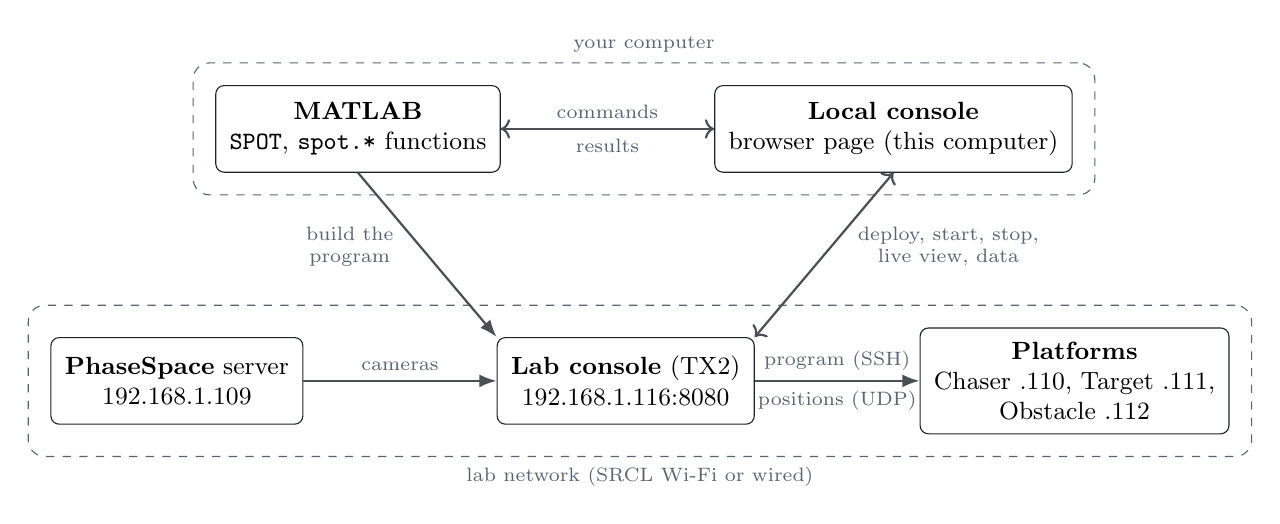
\begin{tikzpicture}[
  box/.style={draw=ink, rounded corners=3pt, align=center, font=\small, inner sep=5pt, minimum height=1.1cm, minimum width=3.2cm},
  arr/.style={-{Latex[length=2.2mm]}, thick, color=ink!80},
  lbl/.style={font=\scriptsize, color=muted, align=center}]
  \node[box] (matlab) at (-3.4, 0) {\textbf{MATLAB}\\ \fn{SPOT}, \fn{spot.*} functions};
  \node[box] (local) at (3.4, 0) {\textbf{Local console}\\ browser page (this computer)};
  \node[box] (tx2) at (0, -3.2) {\textbf{Lab console} (TX2)\\ 192.168.1.116:8080};
  \node[box] (ps) at (-5.7, -3.2) {\textbf{PhaseSpace} server\\ 192.168.1.109};
  \node[box] (plat) at (5.7, -3.2) {\textbf{Platforms}\\ Chaser .110, Target .111,\\ Obstacle .112};
  \draw[arr, <->] (matlab) -- node[lbl, above]{commands} node[lbl, below]{results} (local);
  \draw[arr] (matlab.south) -- node[lbl, left, pos=0.45, xshift=-6pt]{build the\\ program} (tx2.north west);
  \draw[arr, <->] (local.south) -- node[lbl, right, pos=0.45, xshift=6pt]{deploy, start, stop,\\ live view, data} (tx2.north east);
  \draw[arr] (ps) -- node[lbl, above]{cameras} (tx2);
  \draw[arr] (tx2) -- node[lbl, above]{program (SSH)} node[lbl, below]{positions (UDP)} (plat);
  \begin{scope}[on background layer]
    \node[draw=muted, dashed, rounded corners=6pt, fit=(matlab)(local), inner sep=8pt, label={[lbl]above:your computer}] {};
    \node[draw=muted, dashed, rounded corners=6pt, fit=(ps)(tx2)(plat), inner sep=8pt, label={[lbl]below:lab network (SRCL Wi-Fi or wired)}] {};
  \end{scope}
\end{tikzpicture}
\caption{Your computer runs MATLAB and the local console. On the lab network, the lab console (TX2) builds
your program, sends it to the platforms, streams PhaseSpace positions to them, and collects their data.}
\end{figure}

\subsection*{The Project Folder}
Each project is a copy of the SPOT template folder, \pth{template}, made with the MATLAB function
\fn{New\_SPOT\_Project} (Section~\ref{sec:newproject}), which puts it in \pth{projects}. Its top level is kept short:

\begin{xltabular}{\linewidth}{@{}>{\ttfamily}l X@{}}
\toprule
SPOT.m & Starts the local console (\fn{SPOT}, \fn{SPOT open}, \fn{SPOT stop}). \\
<name>.slx & The Simulink diagram, named after the project (the template's \pth{Template\_\allowbreak{}v5\_0\_0\_2026a\_\allowbreak{}Jetson\_\allowbreak{}PSClock.slx}); edit it for your own experiment. \\
SPOT\_User\_Parameters.m & Your own workspace variables; runs after the console's settings are applied. \\
spot\_settings.json & The console's settings, saved automatically. \\
+spot/ & All of SPOT's code, as MATLAB packages (Appendix~\ref{app:functions}); \pth{+spot/+console} also holds the consoles' web code. \\
resources/ & The PhaseSpace marker calibration, the arm calibration script, the reference pictures the console shows. \\
Saved Data/ & Experiment data and saved simulations (the console creates it when it first saves something). \\
SPOT\_Tutorial.pdf & This guide. \\
\bottomrule
\end{xltabular}

% ------------------------------------------------------------------------------------- 2
\section{Setting Up Your Computer}

\subsection{What You Need}

\begin{xltabular}{\linewidth}{@{}l X@{}}
\toprule
\textbf{MATLAB} & \textbf{R2026a or newer} (the template diagram is saved in R2026a; older releases can't open it). \\
For simulations & Simulink, DSP System Toolbox, Control System Toolbox (for the LQR gains). \\
For experiments & Also MATLAB Coder, Simulink Coder, Embedded Coder, and the \emph{MATLAB Coder Support Package for
                  NVIDIA Jetson and NVIDIA DRIVE Platforms} (MATLAB: \ui{Home} $\rightarrow$ \ui{Add-Ons}). \\
\textbf{Python} & 3.6 or newer, standard library only (nothing to \pth{pip install}). It runs the local console's small web server. If it is missing, \fn{SPOT} offers to install it (below). \\
\textbf{Web browser} & Any current browser (Chrome, Firefox, Edge, Brave, Safari). \\
For experiments & A connection to the lab network (SRCL Wi-Fi, or a cable in the lab), and the TX2's password
                  from a lab administrator (needed once). \\
\bottomrule
\end{xltabular}

\subsection{Windows}
\begin{enumerate}
  \item Install MATLAB R2026a with the toolboxes above (MathWorks installer, or \ui{Add-Ons} afterwards).
  \item Python: nothing to do beforehand. If \fn{SPOT} can't find one, it says so and offers \ui{Install Python}, which
        installs it for your user only (with \pth{winget}, or python.org's installer when there is no \pth{winget}; no
        administrator rights needed). To install it yourself: \href{https://www.python.org/downloads/}{python.org}, and
        tick \ui{Add python.exe to PATH}. SPOT tries the Python MATLAB is set up to use (\fn{pyenv}), then \fn{py -3},
        \fn{python}, \fn{python3}, then where the installers put it.
  \item Make your project: run \fn{New\_SPOT\_Project('MyProject')} in MATLAB, from the folder that holds \pth{template}
        (Section~\ref{sec:newproject}). Avoid OneDrive-synced folders while building experiments, since syncing can
        lock files.
  \item Start MATLAB, \ui{cd} into the project folder, and type \fn{SPOT} (Section~\ref{sec:firststart}).
  \item If Windows Firewall asks whether Python may use the network, \emph{private networks} is enough: the local
        console only listens on your own computer (127.0.0.1).
\end{enumerate}

\subsection{Linux}
\begin{enumerate}
  \item Install MATLAB R2026a with the toolboxes above.
  \item Python 3 comes with most distributions. If it is missing, \fn{SPOT} offers \ui{Install Python}, which installs
        it with your package manager (apt, dnf, yum, zypper or pacman) and asks for your password in a system dialog;
        without a desktop it prints the command instead (e.g.\ \pth{sudo apt install python3}).
  \item The local console opens your default browser with \pth{xdg-open} (part of every desktop install).
  \item Make your project: run \fn{New\_SPOT\_Project('MyProject')} in MATLAB, from the folder that holds \pth{template}
        (Section~\ref{sec:newproject}).
  \item Start MATLAB, \ui{cd} into the project folder, and type \fn{SPOT}.
\end{enumerate}

\subsection{A New Project}\label{sec:newproject}
\fn{New\_SPOT\_Project.m} sits next to the \pth{template} and \pth{projects} folders. Run it in MATLAB:
\begin{matlab}
New_SPOT_Project('MyProject')              % creates projects/MyProject, with MyProject.slx
New_SPOT_Project                           % asks for the name
New_SPOT_Project('MyProject', 'D:\SPOT')   % creates D:\SPOT\MyProject instead
\end{matlab}
The name is also the diagram's name, so it must be a valid MATLAB name: letters, digits and \_, starting with a
letter, at most 63 characters, not a keyword and not an existing function. The project is a copy of
\pth{template} with the diagram renamed to \pth{<name>.slx}, this guide, and an empty \pth{Saved Data}; the
template's settings, caches, build files, saved data and documentation are not copied, so the project starts from
the default settings. It prints a link that opens the project and starts the console.
\begin{tipbox}[MATLAB in a Container]
If MATLAB runs in a container (for example with \pth{distrobox}), nothing extra is needed. SPOT fixes the shell
MATLAB uses for \fn{system} when the container doesn't set one, and opens the browser on the host.
\end{tipbox}

\subsection{First Start}\label{sec:firststart}
\begin{enumerate}
  \item In MATLAB, go to the project folder and type:
\begin{matlab}
SPOT          % start the console and open it in your browser
\end{matlab}
  \item MATLAB starts the console's web server, connects to it, and opens the page \ui{SPOT Local Simulations}.
        The address it prints includes a session key: the page only accepts requests from that link.
  \item \fn{SPOT open} opens the page again (for example after closing the tab). \fn{SPOT stop} stops the console.
        Closing MATLAB also disconnects it.
  \item Keep MATLAB open while you use the console: simulations, builds and the page's \ui{MATLAB} command window
        all run in it. The \ui{MATLAB} badge at the bottom of the page says whether it is connected, and what it is doing.
\end{enumerate}

\begin{xltabular}{\linewidth}{@{}>{\raggedright\arraybackslash}p{0.33\linewidth} X@{}}
\toprule
\textbf{If\ldots} & \textbf{then\ldots} \\ \midrule
``needs Python 3.6 or newer'' & Click \ui{Install Python} in the dialog, run \fn{spot.console.installPython}, install it (above), or point MATLAB at it: \fn{pyenv('Version', 'C:\textbackslash ...\textbackslash python.exe')}. \\
The page says it can't talk to MATLAB & Open it with the link MATLAB printed, or run \fn{SPOT open}. \\
The browser doesn't open & Copy the address \fn{SPOT open} prints into your browser. \\
\ui{Lab Disconnected} (top right) & You're not on the lab network. Simulations and results still work; experiments
                                   and the live view need the lab network. \\
The console doesn't start & Its log is \pth{.spot\_cache/console.log} in the project folder. \\
\bottomrule
\end{xltabular}

% ------------------------------------------------------------------------------------- 3
\section{The Local Console (SPOT Local Simulations)}

\subsection{Around the Page}
\begin{itemize}
  \item \textbf{Top bar.} The tabs \ui{Simulation}, \ui{Experiment} and \ui{Results}. Next to them, the
        \ui{Settings} group shows the file your settings are saved to (\pth{spot\_settings.json}) and has three buttons:
        \ui{Load\ldots} (load settings from a \pth{.json}, or an old GUI state \pth{.mat}), \ui{Save As\ldots}
        (save a copy) and \ui{Reset\ldots} (back to the template's defaults, see Section~\ref{sec:settings}).
        On the right: \ui{Lab Console} (opens the hardware console) and the lab badge (\ui{Lab Connected} /
        \ui{Lab Disconnected}).
  \item \textbf{3D view.} The table, the platforms and their paths. Its toolbar has \ui{3D}/\ui{Top}/\ui{Side} views,
        \ui{Initial Conditions} (\ui{Off}, \ui{Initial} or \ui{Home}: which target poses to show on the table),
        \ui{Labels} (name tags and +X/+Y/+Z labels) and \ui{Axes} (each platform's body axes: +X red, +Y green, +Z blue).
        Drag to orbit, right-drag to pan, scroll to zoom.
        The \ui{ZED2 Viewpoint} switch opens a window in the corner showing what the Chaser's ZED2 camera sees, with the
        ZED2's default HD720 intrinsics (1280\,$\times$\,720, $f_x = f_y \approx 528$\,px, 68.6$^\circ$ vertical field of
        view), from the centre of its \ui{Left} or \ui{Right} lens, or \ui{Both} side by side (120\,mm apart, 0.28\,m up
        on its front face, the right lens 0.08\,m right of centre, facing along its +X). It follows the Chaser live, in a
        replay or at its initial conditions, as the window's title says.
        The table is drawn as in the lab: the 0.33\,m granite on its stand (a leg under each corner, painted the barrier's dark grey), with
        the barrier round its edges (from its CAD), lit from the ceiling, so a platform's shadow falls right under it.
        \ui{Use CAD} draws the platforms from the lab's CAD instead of cubes: the Chaser in silver MLI with its ZED2
        (Stereolabs' ZED~2i model, the ZED~2's housing, in a cutout of its size), the Garmin LIDAR-Lite behind the
        front panel's two small holes, and arm; every platform also shows its eight thrusters (Silvent MJ4 nozzles in
        black PLA inserts in the side panels' bottom notches), the LED mounts at its top corners and the countersunk
        black Phillips screws in its panels and aluminium frame (the links follow the joint angles in a replay), the Target in gold MLI, each with the docking cone and solar panels set in the Spacecraft Designer (Section~\ref{sec:designer}), and
        the Obstacle as an aluminium frame with transparent blue plexiglass panels on its sides and top (every platform has its internal structure). The models are solid; a simulation laid over the live view is
        see-through with an outline, and loaded results are faint with a dashed outline.
        The models are made from the lab's SolidWorks assemblies by \pth{build\_cad\_models.py}, which lives outside the
        template, with the CAD it reads (\pth{designs/cad\_tools}); run it again after changing the CAD.
  \item \textbf{Messages} (right, on the Simulation and Experiment tabs). Each platform's debug message, in three
        parts (RED, BLACK, BLUE): the text the diagram writes to \fn{RED\_Logger}, \fn{BLACK\_Logger} and
        \fn{BLUE\_Logger}, e.g.\ ``Chaser: Running Phase 1''. Only changes are listed, with their time and, when a
        message came several times in a row, how often (\ui{$\times$30}). After a simulation they are the
        simulation's messages, and the replay highlights the one in effect; during an experiment they come live from
        the platforms (in a diagram with the shared PhaseSpace clock), so a simulation shows what the experiment will.
        The arrow tucks the panel away to give the 3D view more room.
  \item \textbf{MATLAB command window} (bottom), with two tabs. \ui{MATLAB}: type MATLAB commands. They run in your MATLAB session's
        workspace (Enter runs, Shift+Enter starts a new line, $\uparrow$ recalls earlier commands). Its tab shows what MATLAB is doing (\ui{Idle}, or e.g.\ \ui{running the simulation}); the arrow on the right collapses the window.
        \ui{Live Plot} (Simulation and Experiment tabs): plots the signals the diagram's \emph{Live Stream} blocks send, live in simulations and
        experiments. \ui{Data Available to Stream} lists them, each named after what is connected to its block (e.g.
        \fn{RED\_Measured\_States}); tick one to plot it, and choose its elements with the \ui{1}~\ui{2}~\ldots\ chips.
        The window (\ui{10\,s} to \ui{All}), \ui{Pause} and the readout under the mouse help to read it; after a
        simulation the replay's time is marked. To stream another signal, copy a Live Stream block in the diagram's
        \emph{Live Data Streams} subsystem and connect a Data Store Read (or any signal) to it.
\end{itemize}

\subsection{Simulation Tab}
The sidebar has five tabs. Every change is sent to MATLAB at once and saved. MATLAB puts the settings into the
base workspace as the diagram expects them, then runs \pth{SPOT\_User\_Parameters.m}.

\begin{description}[leftmargin=1em]
  \item[Scenario.]
    \begin{itemize}
      \item \ui{Diagram}: which \pth{.slx} in the project folder to use. \ui{Open in Simulink} opens it in MATLAB.
      \item \ui{Platforms}: Chaser, Target, Obstacle and Arm (the arm on the Chaser).
      \item \ui{Sample Rate}: the controller rate, in Hz. The diagram's step is 1/rate.
      \item \ui{Data Rate}: the PhaseSpace data rate, in Hz: how often the cameras send the platforms' positions in an
            experiment (\texttt{dataRate} in the settings file; whole Hz, 1 to 960; 10 by default). It is the Experiment
            tab's \ui{Data Rate} too, and \emph{locked}: the padlock beside it unlocks it, after a warning, on both tabs
            (the page locks it again when reloaded). The diagram's \texttt{dataRate} variable is its period,
            1/\texttt{dataRate}\,s; the LQR gains are designed at it and the measured states come at it, so build again
            after changing it.
      \item \ui{Thruster PWM}: the thrusters' PWM frequency, in Hz (\texttt{PWMFreq} in the diagram; 5 by default). The
            duty cycles assume a valve period of 1/frequency. The Teensy firmware runs its own PWM at 5\,Hz
            (\texttt{PWM\_FREQUENCY} in \pth{+spot/+hardware/teensy/teensy\_pwm\_control.ino}): change both, or the
            simulation warns. It is \emph{locked} like the data rate: its padlock explains this before it unlocks.
      \item \ui{Calibrated Thrust}: use each thruster's measured thrust (on by default; the lab's thruster calibration,
            Section~\ref{sec:calibration}) in the diagram's mixer, and so in the simulated plant and in experiments
            built from the project. Off, or without a calibration, every thruster gives the Platforms tab's
            \ui{Thrust}, which says which is used.
      \item \ui{Calibrated Arm}: use the arm's measured friction and inertia (on by default; the lab's arm calibration,
            or a \pth{resources/arm\_calibration.json} copied by hand: the newer). Off: the arm model's defaults.
      \item \ui{Table Slope}: simulate the table's measured slope (on by default): the floating platforms slide
            downhill, and their air bearings drag them, as the lab's table slope calibration found
            (Section~\ref{sec:calibration}; the project's \pth{resources/spot\_calibration.json}). The line beside it says
            what the project has. Off, or without a calibration, the table is level.
      \item \ui{Timeline}: the phases. Phase 0 synchronizes, 1 starts floating, 2 moves to the initial pose, 3 is the
            experiment (sub-phases 3.1--3.4), 4 returns home and 5 holds there.
            Type each duration in seconds. The switches (or a click on a segment of the bar) \emph{skip} phase 2,
            any sub-phase or phase 4. A skipped segment takes no time, in simulation and in experiments.
            Phases 0, 1 and 5 always run (they switch the platforms on and off).
    \end{itemize}
  \item[Platforms.] Pick the Chaser, Target, Obstacle or Arm.
    \begin{itemize}
      \item \ui{Initial Conditions}: where each platform starts (\ui{Initial}: the simulation starts here and phase~2
            drives the platform here) and where it returns (\ui{Home}), as x\,[m], y\,[m], $\theta$\,[$^\circ$].
            Click \ui{Initial} or \ui{Home} to show those poses on the table, then drag a platform to move it
            (Shift+drag rotates it).
      \item \ui{Mass Properties}: the three scale readings A, B, C [kg] and the bifilar-pendulum test (T, L, D) give
            the mass, the centre of gravity and the inertia (pictures in \pth{resources/}).
            \ui{Override} uses a mass and inertia you type instead.
            \ui{Thrust} is the force of one thruster.
      \item \ui{Thruster Offsets and LED Positions}: the computed geometry. \ui{Write PhaseSpace Marker File} writes
            \pth{resources/tracker\_positions\_phasespace.txt}, which the Experiment tab sends to PhaseSpace before streaming.
      \item For the arm: its \ui{Initial Pose} (shoulder, elbow, wrist angles), geometry, link masses and inertias
            (\pth{resources/ArmConfig.png}).
    \end{itemize}
  \item[Control.] One LQR per platform. A row per axis (x, y, $\theta$) holds its \ui{Error Q}, \ui{Rate Q} and
        \ui{Effort R} weights. A larger Q corrects that error harder; a larger R uses the thrusters more gently.
        \ui{Gain K (Computed)} shows the resulting gain matrix. With the Arm on, two more cards set the arm's
        position and velocity controllers (Section~\ref{sec:arm}): P, I, D per joint (the servos' own units),
        the profile and the PWM limit (\texttt{control.ARM} in the settings, \texttt{armControl} in MATLAB).
  \item[Solver.] Fixed-step or variable-step, and its options. They are read from the diagram when you choose it, and
        used for simulations without changing the diagram file.
  \item[Workspace.] MATLAB's base workspace: click a variable to inspect it (values, struct fields, or a plot for a
        time series).
\end{description}

\paragraph{Your First Simulation.}
\begin{enumerate}
  \item On \ui{Scenario}, check the diagram, switch on \ui{Chaser}, and leave the timeline as it is.
  \item On \ui{Platforms}, look at the Chaser's initial and home poses (show them with \ui{Initial Conditions: Initial}).
  \item Click \ui{Run Simulation} (with \ui{Real Time} on, it runs at the clock's pace, one second of simulation per
        second, to watch the Live Plot, the messages and the 3D view as during an experiment). The status line shows the progress, and \ui{Run Simulation} becomes \ui{Stop}
        while it runs. Simulink's messages go to the command window, not MATLAB's (warnings can be expanded there).
        If the simulation fails, the status line gives the root cause and the block it is in; \ui{Details} opens the
        whole chain of causes, the line in your own code (e.g.\ \pth{SPOT\_User\_Parameters.m}), what Simulink printed
        before failing and MATLAB's full report in the command window, and \ui{Show Block} opens the diagram at the
        block, highlighted.
  \item When it finishes, the replay starts in the 3D view. The playback bar has play/pause (also the space bar),
        a scrub bar with the phase boundaries, the current phase, the speed, and \ui{Paths}. Paths are traced behind
        the platforms as they move.
  \item \ui{Save Results} (next to \ui{Run Simulation}) keeps this run, with the settings it ran with, in
        \pth{Saved Data/Simulation\_<diagram>\_<date\_time>/}, to replay or plot later.
        Until then the run is only in MATLAB's workspace (\fn{dataClass}, \fn{simOut}).
\end{enumerate}

\paragraph{Comparing Runs on the Table.}
\ui{Compare} (in the playback bar) lays other results over the simulation: experiment runs, saved simulations, or
copies of earlier runs.
\begin{itemize}
  \item \ui{Keep This Simulation} keeps a copy of the current run, so you can compare it with the next one.
  \item \ui{Load Results\ldots} opens the \pth{Saved Data} list.
  \item Each result has a switch and a time offset [s] to line it up. Overlays are drawn with outlined platforms
        and dashed paths, labelled with the result's name.
  \item \ui{Last Simulation} hides or shows the current run.
\end{itemize}

\subsection{Experiment Tab}
The Experiment tab builds the selected diagram on the lab console, deploys it to the platforms, runs it, and collects
the data. It needs the lab network: without it the tab is locked and says so.
It uses the Simulation tab's settings: the diagram, the platforms and the timeline.

\begin{warnbox}
Before starting an experiment, make sure the table is clear, the platforms are where they should be, and the
E-stop is within reach. \ui{Stop} sends ``all off'' to the platforms. Each platform's Teensy also switches
everything off by itself if commands stop arriving for 2\,s.
\end{warnbox}

\begin{enumerate}
  \item \textbf{Lab.} The card shows the lab console and PhaseSpace. \ui{Lab Console (TX2) Address} is the TX2's
        address (\texttt{labConsoleAddress} in the settings file; 192.168.1.116): the page reaches the lab console there,
        experiments are built and deployed through it, and the platforms send it their clocks, debug messages and live
        streams (the diagram's \texttt{labConsoleIP}), so build again after changing it. The cameras' \ui{Data Rate}
        [Hz] is the Scenario's \ui{Data Rate} (the same setting, locked the same way), fixed while the cameras stream.
        \ui{Start Cameras} sends this project's marker calibration (\pth{resources/tracker\_positions\_phasespace.txt})
        and starts streaming at that rate. The platforms then appear live in the 3D view.
  \item \textbf{Platforms.} Each selected platform's state: \ui{Ready} when it answers and its Teensy is free.
        Its bin button takes it out of the experiment (it is switched off in Scenario; the Chaser takes the arm with it).
  \item \textbf{Build}, in three steps.
        \begin{enumerate}
          \item \ui{Check}: loads the diagram and lists what the build will do; nothing is compiled.
          \item \ui{Connect}: connects MATLAB to the TX2. Type its password the first time; MATLAB remembers it.
          \item \ui{Build}: generates the code and compiles it on the TX2 (a few minutes). The build log appears live.
                The diagram file itself is not changed: the build's own settings (plant model commented out, ode4,
                NVIDIA Jetson board, build only) are undone afterwards.
        \end{enumerate}
  \item \textbf{Deploy \& run.}
        \begin{itemize}
          \item \ui{Deploy} copies the program from the TX2 to each selected platform.
          \item \ui{Start Experiment} starts it on all of them (PhaseSpace must be streaming). Each platform's clock
                appears over the 3D view, and the live paths are drawn. Tick \ui{Simulation} there to overlay your
                simulation in step with the experiment's clock.
          \item The template's diagram uses the \emph{shared PhaseSpace clock} (see below): the
                platforms then wait at time 0 until every program is running, and the lab console starts them together
                3\,s later, through the PhaseSpace stream they all receive. The status says what it is waiting for, and
                then how close the platforms' clocks are (``clocks within 4\,ms'').
          \item \ui{Stop} stops it early. Otherwise it ends by itself at the end of phase 5.
        \end{itemize}
        \begin{tipbox}[The Shared PhaseSpace Clock]
        In the earlier template diagram (now in \pth{archive/Legacy/original\_diagram}) each platform broadcast its own
        Simulink clock and followed the last one to start, so the platforms were off by however their programs and
        the Wi-Fi happened to start. In the template's diagram,
        \pth{Template\_\allowbreak{}v5\_0\_0\_2026a\_\allowbreak{}Jetson\_\allowbreak{}PSClock.slx}, the experiment time comes
        from the PhaseSpace stream instead (\fn{spot.hardware.experimentTime}): one clock for every platform, started at
        an agreed moment, and a program started late stays at time 0. Its \emph{Debugger} sends each platform's
        message to the lab console (the Messages panel), and records it in simulations, and its \emph{Live Data
        Streams} subsystem feeds the Live Plot. Every UDP link in it uses
        \fn{spot.hardware.udpSend} / \fn{udpReceive} (the newest packet, never a queue of old ones).
        \end{tipbox}
  \item \textbf{Data.} \ui{Collect} copies each platform's log files into \pth{Saved Data}, in a folder named
        after the diagram and the time with one subfolder per platform. It converts them to MATLAB time series
        (\pth{<PLATFORM>\_<n>.mat}, variable \fn{dataClass\_rt}) and saves the settings next to them.
        Open them on the Results tab.
\end{enumerate}
\begin{tipbox}
If you change the timeline, the platforms or the diagram, build again: the settings are part of the program.
\end{tipbox}

\subsection{Results Tab}
\begin{enumerate}
  \item \textbf{Load data} (\ui{Datasets} card).
        \begin{itemize}
          \item \ui{Last Simulation} takes a copy of the current run.
          \item \ui{Saved Data\ldots} lists experiment runs (``Run 1'', ``Run 2'' for each start) and saved simulations,
                newest first. Runs whose log files weren't converted yet have a \ui{Convert ExpLog Files} button.
          \item \ui{Open .mat\ldots} opens any file of logged signals.
        \end{itemize}
        Each dataset's \ui{3D} button replays it on the Simulation tab, over the simulation.
  \item \textbf{Plot.} Click a dataset, then click its signals (grouped Chaser, Target, Obstacle, Arm, other) to add them to the
        selected plot; click again to remove. Multi-column signals (e.g.\ \fn{Duty\_Cycle}) have a button per column.
        \begin{itemize}
          \item \ui{+ Plot} adds a plot below. Each plot has one y axis and up to eight lines, and lines from
                different datasets can share a plot.
          \item The \ui{x} menu plots against another signal instead of time. A platform's \fn{Py\_m} against \fn{Px\_m}
                draws its path on the table; tick \ui{Equal} for true shapes.
          \item Hover to read values. Drag across a plot to zoom; double-click to zoom out. \ui{Axes} sets the limits.
                \ui{Link Time} zooms and hovers the time plots together. \ui{Smoothing} applies a Gaussian filter.
        \end{itemize}
  \item \textbf{Export} (\ui{Export} menu). MATLAB draws the plots in the lab's publication style: Times, the
        platforms' colours (Chaser grey-silver, Target gold, Obstacle blue, named so in the legend), every sample, and table plots with the platforms' outlines.
        \begin{itemize}
          \item \ui{Save PDF\ldots} saves a PDF, EPS, SVG or 700\,dpi PNG; choose its width, height and font size first.
          \item \ui{Open in MATLAB} opens it as a figure you can adjust.
        \end{itemize}
\end{enumerate}

\subsection{Settings and Your Own Parameters}\label{sec:settings}
\begin{itemize}
  \item The settings are saved to \pth{spot\_settings.json} after every change. Use \ui{Save As\ldots} to keep
        versions, and \ui{Load\ldots} to go back to one. \ui{Load\ldots} also reads a state saved by the old SPOT GUI.
  \item \ui{Reset\ldots} starts from a clean slate, in parts you choose.
        \begin{itemize}
          \item \emph{Simulation settings}: back to the template, keeping your diagram.
          \item \emph{Page and view}: the page's own preferences.
          \item \emph{Loaded results}: closes the loaded datasets.
        \end{itemize}
        The settings file is backed up to \pth{.spot\_cache/settings\_before\_reset\_<time>.json} first, so
        \ui{Load\ldots} can bring it back.
  \item Put variables of your own in \pth{SPOT\_User\_Parameters.m}. It runs every time the settings are applied
        (and before every simulation and build), so it can also override any of SPOT's values.
\end{itemize}

\subsection{Spacecraft Designer}\label{sec:designer}
The \ui{Designer} tab, on both consoles, sets what is mounted on each platform. The 3D view shows the chosen
platform's CAD model close up at the centre of the table; drag to orbit, scroll to zoom.
\begin{itemize}
  \item Pick the platform (\ui{Chaser}, \ui{Target}, \ui{Obstacle}) at the top of the sidebar.
  \item \ui{Docking Cone}: \ui{None}, \ui{Male} (the cone that goes in, on the interface bracket, with the steel disk
        at its tip) or \ui{Female} (the cup with the electromagnet at its bottom, on an arm coupler's plate). By default
        the Chaser has the male cone and the Target the female one, both at the left of their +Y face, as in the lab.
  \item On the Chaser, \ui{Arm} mounts the robotic arm instead: on an arm coupler's plate (the female cup's bracket),
        with the male docking cone as its end effector, so it is the arm or a cone, never both. The place you pick is
        the arm's mount, and the view shows the whole arm at its initial pose. On the local console this is the same
        choice as the Simulation tab's \ui{Arm} platform: picking \ui{Arm} turns it on (and the simulation mounts the arm
        at that place), another choice turns it off, and switching the \ui{Arm} platform on or off picks or drops it
        here (a dropped arm gives the Chaser back its male cone).
  \item Its place is one of 6: the +X (front, where the Chaser's ZED2 is), +Y or $-$Y face (not the back, $-$X, where
        the control panel is), and the left or right of the face as seen from outside, in the upper half. The places are symmetric about the face's
        vertical centre line (the arm coupler's place, mirrored). Click a place on the face map (each face drawn as
        seen from outside, with the faces its edges meet) or a disc on the model.
  \item On the Chaser, the orange place is the arm's usual one (the arm coupler); a cone there, on its own bracket,
        takes its place. The side panels follow the cone (or the arm): each
        face's panel has the cutout for the cone's bracket only where the cone is, so moving the cone leaves no
        empty cutout behind. Red, dashed places would be blocked by something
        that stands out of the face; you can still choose them, with a warning.
  \item \ui{Solar Panels}: \ui{Include} adds the pair of panels on their bracket over the top, standing off the
        $\pm$X faces (\ui{Along X}) or the $\pm$Y faces (\ui{Along Y}). The bend in one of the bracket's legs goes round
        the control panel (on $-$X). Each frame carries a 1\,mm panel on each side, drawn as the lab's panels look (the
        CAD has the frames only): a white backsheet with rounded corners and an eyelet in each, round a field of
        9\,$\times$\,8 black monocrystalline cells with thin silver lines between them.
\end{itemize}
Each console keeps one design: the local console in \pth{spot\_design.json} in the project folder, the lab console
on the TX2. Every change is saved at once, and every 3D view of that console draws it whenever \ui{Use CAD} is on.
On the local console, the \ui{Lab Console} card says whether the lab console's design is the same, and offers
\ui{Send to Lab Console} and \ui{Use Lab Console's Design}.

% ------------------------------------------------------------------------------------- 4
\section{The Hardware Console (SPOT Hardware Interfaces)}

On the lab network, open \pth{http://192.168.1.116:8080} (or click \ui{Lab Console} in the local console, which follows
the Experiment tab's \ui{Lab Console (TX2) Address}).
It always runs on the TX2 and starts by itself when the TX2 boots. Everyone in the lab sees the same state: if
someone else starts the cameras or switches a thruster on, your page shows it too.

\subsection{PhaseSpace Tab}
\begin{itemize}
  \item \ui{Compile} builds the PhaseSpace streamer (StreamData) on the TX2. It's only needed after StreamData's source
        changes, since \pth{deploy\_tx2.sh} already compiles it.
  \item \ui{Stream}: choose a \ui{Frequency} [Hz] and \ui{TCP} or \ui{UDP} (UDP drops a late frame instead of delaying
        the next ones), then \ui{Start Streaming}. The platforms receive the positions on UDP port 31534.
        \ui{Destinations} adds other computers that should receive them; \ui{+ This Computer} adds yours.
  \item \ui{Telemetry} lists each platform's position, attitude and rates, and the LEDs PhaseSpace can see. The 3D
        view shows the platforms and LEDs live (\ui{LED IDs} numbers them; \ui{LED Height Lines} draws a line from each LED down to the table).
\end{itemize}
The Experiment tab of the local console starts and stops the cameras for you, at the right rate, with your
project's marker calibration.

\subsection{Interactive Mode}
Fly platforms by hand: drag where each should go on the table, and the console flies them there with the
template diagram's own controller, several at once if you like.
\begin{enumerate}
  \item Start streaming, and check on the Hardware tab that the platforms are \ui{Ready}.
  \item Switch on \ui{Interactive Mode} (below \ui{Telemetry}). It has a row for the \ui{Chaser}, \ui{Target} and
        \ui{Obstacle}, each with a switch: switch on the ones to fly (or click them in the 3D view). Each one's
        \emph{goal} appears on top of it, a dashed outline in its colour.
  \item Drag each goal where its platform should go; Shift+drag turns it. \ui{Here} puts it back on the platform.
  \item \ui{Fly to Goals}: every switched-on platform's pucks come on and they all fly to their goals at once.
        Keep dragging a goal and its platform follows. Switch on another platform during the flight and
        \ui{Fly to Goals} adds it.
  \item A platform's switch stops that platform (everything on it off); \ui{Stop All} or \textbf{Esc} stops them all.
\end{enumerate}
Each row shows the platform's goal, how far it still is from it, and each thruster's duty cycle; the 3D view
draws the gas leaving the nozzles that fire.

Every \texttt{baseRate} (0.05\,s at the default 20\,Hz, as often as the diagram's controller and thruster code
run), the TX2 takes each platform's pose and velocity from PhaseSpace, computes the forces with the default LQR
law and the thrusters' duty cycles with the diagram's mixer, and sends them to its Teensy. Each platform has its
own loop and its own controller process, so the platforms run side by side on the TX2's CPU cores. The law and
the mixer are \fn{spot.control.lqrCommand} and \fn{spot.control.thrusterDutyCycles}, which hold verbatim copies
of the blocks' code, ported line by line to Python (\pth{+spot/\allowbreak{}+console/\allowbreak{}webapp/\allowbreak{}spot\_console/\allowbreak{}control.py})
because the TX2 has no MATLAB. In MATLAB, \fn{spot.control.\allowbreak{}verifyConsoleController} checks that the
copies are still the diagram's code, that they reproduce a simulation of the diagram step by step, and that the
Python agrees with MATLAB. The gains and mass properties are SPOT's defaults (\ui{Controller} in the card lists them).
\begin{warnbox}
The platforms really fly. Clear the table first, and keep a hand near \textbf{Esc}.
\begin{itemize}
  \item Each platform flies straight at its goal and knows nothing of the others. Goals must be at least
        0.45\,m apart (centre to centre), and away from platforms resting on the table, but the paths can still
        cross: place the goals so they don't.
  \item Everything on \emph{one} platform goes off when PhaseSpace loses it (1\,s), when it is seen off the
        table, when its link or Teensy is taken (an experiment, another program), or when someone switches it off
        on the Hardware tab. The others fly on.
  \item Everything on \emph{every} platform goes off when the page that started the flight closes or loses the
        network (3\,s), or on \ui{Stop All} / \textbf{Esc}.
  \item Goals stay 0.2\,m inside the table's edges. Any page can stop a flight; only the page that started it can
        move its goals or add platforms. The Hardware tab's buttons for a flying platform are locked meanwhile.
\end{itemize}
\end{warnbox}

\subsection{Hardware Tab}
Each platform has a card.
\begin{itemize}
  \item \ui{Pucks} switches its air bearings on or off.
  \item The eight thruster buttons fire one thruster each, at the duty cycle set beside them.
  \item \ui{Thruster Check} fires them one after the other, for the time set per thruster.
  \item \textbf{Esc} switches everything off on every platform.
\end{itemize}
Commands go to each platform's Teensy over SSH. The Teensy switches everything off when commands stop for 2\,s, so
nothing stays on if the page or the TX2 goes away. While an experiment uses a platform's Teensy, its card is locked.

\subsection{For Lab Administrators}
These one-time scripts live in \pth{+spot/+console/deploy/} and \pth{+spot/+hardware/teensy/}. Run them from a
computer whose SSH key the TX2 and the platforms accept, and start the path with \pth{./} (bash reads a path
starting with \texttt{+} as an option).
\begin{xltabular}{\linewidth}{@{}>{\ttfamily\raggedright\arraybackslash}p{0.36\linewidth} X@{}}
\toprule
./\allowbreak{}+spot/\allowbreak{}+console/\allowbreak{}deploy/\allowbreak{}deploy\_tx2.sh & Copy the console to the TX2, compile StreamData there, and (re)start its
                                        service. Run it after any change to the console. \\
./\allowbreak{}+spot/\allowbreak{}+console/\allowbreak{}deploy/\allowbreak{}setup\_hardware\_link.sh & Install the platform agent on RED/BLACK/BLUE and give the TX2's key
                                        access to it (only to it). \\
./\allowbreak{}+spot/\allowbreak{}+hardware/\allowbreak{}teensy/\allowbreak{}setup\_teensy\_serial.sh & Make each platform's Teensy serial port usable without sudo. \\
\bottomrule
\end{xltabular}

\subsection{Calibration Tab}\label{sec:calibration}
Measurements of the lab that make simulations behave as the experiments do. The lab console runs them and keeps the
lab's calibration (\pth{\textasciitilde/.spot\_calibration.json} on the TX2); each project keeps a copy,
\pth{resources/spot\_calibration.json}, which its simulations use. Three calibrations: \ui{Table Slope},
\ui{Thrusters} and \ui{Arm}.

\paragraph{Table Slope.} The table isn't perfectly level, so a floating platform slides downhill. With PhaseSpace
streaming and the platform resting on the table, the calibration
\begin{enumerate}[nosep]
  \item records the platform resting for 2\,s (the cameras' noise);
  \item floats it with the thrusters off, and records it drifting from where it is;
  \item flies it (the diagram's own controller, as Interactive Mode) to each point of a grid over the table, lets it
        settle, switches the thrusters off and records it drifting again;
  \item fits the table's height surface (a smooth quadratic surface, or a plane when the drifts don't cover enough
        of the table) and the air bearings' drag to every drift.
\end{enumerate}
Choose the platform, the grid (3\,$\times$\,2 by default), the drift time (12\,s), the edge margin (0.35\,m) and the
model, then \ui{Start Table Calibration}; the default takes about 4 minutes. The map then shows the table's height
in colour (blue low, red high), its contour lines, which way is downhill and the drifts; below it, the tilt at the
centre and the steepest (in mrad: 1\,mrad is a 1\,mm drop per metre), the downhill direction, and how well the
model fits. The 3D view's \ui{Table Slope} switch colours the table top the same way.

\begin{warnbox}
\begin{itemize}[nosep]
  \item A drift ends at once (pucks off: the platform stops on its pucks) when the platform comes within the edge
        margin of an edge, within 0.45\,m of another platform, or goes faster than 0.15\,m/s. Grid points next to
        other platforms are skipped; clear the table around the grid.
  \item \ui{Stop} or \textbf{Esc} on the tab ends it with everything off; so does Esc or switching the platform off
        on the Hardware tab (where it shows as \emph{Calibrating}), PhaseSpace losing it for 1\,s, or the link to it
        dropping. Experiments and Interactive Mode can't start while it runs, nor it while they do.
\end{itemize}
\end{warnbox}

\paragraph{Thrusters.} Each thruster's real thrust. With PhaseSpace streaming and the platform resting on the table,
for each thruster 1 to 8 (and each repeat) the platform floats where it rests, the thruster fires at full thrust for
the burn time (2\,s by default), the diagram's controller flies it back to where it started, and the pucks go off
for a moment's rest. Each burn's thrust is the platform's mass times the acceleration it gave (the table's slope,
from the table calibration, taken out), so it is only as good as the platform's mass, inertia and centre of
gravity: before it starts, a dialog shows the values the lab console assumes (SPOT's defaults), lets you change them
for this run, and asks you to confirm. The result shows each thruster's thrust against nominal (bars with their
spread, and arrows on the platform showing which way each really pushes), and a \emph{torque ratio}: the turn each
burn gave against the turn its thrust should give, which is far from 1 when the CG or the inertia is off. The lab
console's controller (Interactive Mode) uses the calibrated thrust at once.

\paragraph{Arm.} The arm's friction and inertia, with the real servos: the tab runs \pth{calibrate\_arm.py} (Section~\ref{sec:arm})
on the Chaser through its agent. Opening \ui{Arm} checks what the script needs there (Python~3, the Dynamixel SDK, the
U2D2 at \pth{/dev/ttyUSB0} and access to it, nothing else holding it), item by item with what to do about each. Pick
the joints and tests, then \ui{Start Arm Calibration}; a dialog asks you to confirm the Chaser rests on the table and
the arm is clear (each joint moves up to 25$^\circ$). The console keeps the Chaser resting meanwhile; \ui{Stop} (or
Esc) switches the servos' torque off at once. The result shows each joint's friction (its breakaway torque, and the
friction against speed with the fitted curve), its inertia, and its position steps. \ui{Rehearse (Simulated Servos)}
runs the script's simulated servos instead: no hardware needed, and the result is never saved as the lab's.

\paragraph{On the local console.} The Calibration tab shows the project's calibration next to the lab's, with
\ui{Update from Lab}. Whenever your computer is on the lab network and the lab's calibration is newer, the page asks
once: \ui{Update} copies it into the project, \ui{Not Now} keeps the project's (and doesn't ask again until the lab's
changes), and \ui{Never Ask Again} stops asking for this project (the tab's \ui{Ask When the Lab's Is Newer} turns it
back on). The Simulation tab's \ui{Table Slope}, \ui{Calibrated Thrust} and \ui{Calibrated Arm} use it.

% ------------------------------------------------------------------------------------- 5
\section{Running Simulations Without the GUI}
Everything the console does is an ordinary MATLAB function (Appendix~\ref{app:functions}), so you can script it:
for batch runs, parameter sweeps, or when you just prefer the Command Window. Run these from the project folder.

\subsection{One Simulation}
\begin{matlab}
root = pwd;                                     % the project folder
s = spot.params.load('spot_settings.json');     % the console's settings (or spot.params.defaults())
s.diagram = 'Template_v5_0_0_2026a_Jetson_PSClock.slx';
s.platforms.RED = true;  s.platforms.BLACK = false;
s.timing.subPhases = [10 10 30 60];             % phase 3 sub-phases [s]
s.timing.on.phase4 = false;                     % skip phase 4
s.initial.RED.initial = [2.0 1.2 90];           % x [m], y [m], theta [deg]
s.control.RED.lqr.Q = [2 2 0.1 10 10 1];        % x y theta dx/dt dy/dt dtheta/dt
s.solver = spot.sim.readSolver(s.diagram, root, s.solver);   % the diagram's own solver
out = spot.sim.run(s, root);                    % simulates; dataClass is in the workspace
fprintf('%g s simulated in %.1f s\n', out.tsim, out.seconds);
\end{matlab}
\fn{spot.sim.run} applies the settings, runs \pth{SPOT\_User\_Parameters.m}, simulates without modifying the
diagram file, and leaves \fn{dataClass}, \fn{dataPacket} and \fn{simOut} in the base workspace, as the old GUI did.
The settings are an ordinary struct: see \fn{spot.params.defaults} for every field and its unit.

\subsection{Looking at the Results}
\begin{matlab}
plot(dataClass.RED_Px_m); hold on; plot(dataClass.RED_Px_Desired_m)   % timeseries
spot.data.saveSimulation(s, root);              % keep it in Saved Data (with s)

% A figure in the lab's publication style, saved as PDF
ds = spot.data.load(struct('source', 'simulation'), root, s);   % a copy of this run
lookup = @(id) ds{1};
panel = struct('traces', struct('id', 'sim', 'signal', {'RED_Px_m', 'RED_Px_Desired_m'}, 'col', 1));
fig = spot.data.toFigure({panel}, lookup);
spot.data.exportFigure(fig, fullfile(root, 'red_x.pdf'));
\end{matlab}
A panel whose \fn{x} is \fn{struct('signal', 'RED\_Px\_m', 'col', 1)}, with \fn{RED\_Py\_m} as its trace,
draws the Chaser's path on the table, with its outline at the start and the end. Experiment runs load the same way:
\fn{spot.data.listSaved(root)} lists them, and \fn{spot.data.load} reads one (its help explains the
\fn{files} and \fn{file} forms).

\subsection{From a Terminal (Batch)}
MATLAB's \fn{-batch} option runs a command without the desktop, and exits when it ends. The same line works on Windows
(Command Prompt or PowerShell) and Linux:
\begin{shell}
matlab -batch "cd('C:/Users/you/SPOT/MyProject'); s = spot.params.load('spot_settings.json'); spot.sim.run(s, pwd); spot.data.saveSimulation(s, pwd);"
\end{shell}
For anything longer, put the commands in a script (e.g.\ \pth{my\_runs.m} in the project folder) and run
\pth{matlab -batch "my\_runs"}.

\subsection{A Parameter Sweep}
\begin{matlab}
root = pwd;
s = spot.params.load('spot_settings.json');
s.solver = spot.sim.readSolver(s.diagram, root, s.solver);
for q = [0.5 1 2 4]
    s.control.RED.lqr.Q(1:2) = q;               % position weights
    out = spot.sim.run(s, root);
    folder = spot.data.saveSimulation(s, root); % each run in its own Saved Data folder
    fprintf('Q = %g: saved in %s\n', q, folder);
end
\end{matlab}
The saved runs then appear in the Results tab's \ui{Saved Data\ldots} list, ready to plot or replay side by side.

\subsection{Experiments from MATLAB}
Building works from MATLAB too, on the lab network:
\begin{matlab}
p = spot.experiment.plan(s, root);              % what the build would do (no compiling)
spot.experiment.connect(root, 'tx2-password');  % once; afterwards spot.experiment.connect(root)
out = spot.experiment.build(s, root);           % generates the code and compiles it on the TX2
\end{matlab}
Deploying, starting, stopping and collecting the data are done by the lab console: use the local console's
Experiment tab (or the hardware console) for those steps.

% ------------------------------------------------------------------------------------- execution order
\section{The Arm: Servos, Friction and Calibration}\label{sec:arm}
The Chaser's arm has three Dynamixel MX servos (shoulder, elbow, wrist; IDs 1, 2, 3). Their gearboxes have a lot of
friction: a joint takes a firm push to start moving, a small torque command doesn't move it at all, and the arm stays
still while the platform flies.

The servos run in \textbf{current control} for the whole experiment: the diagram sends each joint a torque, and the
servo holds the motor current that gives it. Position and velocity control are controllers in the diagram that run the
servos' own control laws (the ones the servos run in their position and velocity modes) and give torques. In
simulation the plant stands in for the arm, with the same inputs and outputs.

\subsection{How the Arm Is Simulated}
The diagram's \ui{Simulate Plant Dynamics / RED and ARM Dynamics / RED + ARM} holds one block, \ui{RED + ARM Plant}
(\fn{spot.arm.Plant}). Every step of the diagram (1/\ui{Sample Rate}, e.g.\ 50\,ms), it takes 1\,ms steps of its own of:
\begin{itemize}
  \item \textbf{The servos} in current control, with the torques the diagram sends (\fn{ARM\_Controls}, N\,m): each
        becomes a goal current as the hardware block converts it (torque / torque constant, in 3.36\,mA steps, within
        the Current Limit), and the servo holds that current as far as its supply voltage allows (the motor's
        back-EMF), from the datasheet's stall torque, stall current and no-load speed.
  \item \textbf{The dynamics} of the base and the three joints, coupled, with each joint's rotor inertia.
  \item \textbf{The friction} of each joint (below).
\end{itemize}
Every step it also writes what the hardware block measures: the joint angles at the encoders' resolution and the joint
speeds in the servos' velocity units (\fn{ARM\_Measured\_States}), and the torques the servos report
(\fn{ARM\_Measured\_Torque}). The rest of the diagram keeps its own rate: a 275\,s simulation of all three platforms
and the arm takes about 10\,s.

\subsection{The Arm's Controllers}
\ui{3 - Control} picks the arm's controller from \fn{ARM\_Control\_Law\_Enabler}, which each phase of
\ui{1 - Experiment Logic} sets (Table~\ref{tab:armctl}). Each one writes the joint torques to \fn{ARM\_Controls} and
its number to \fn{ARM\_Control\_Mode}.

\begin{table}[h]
\centering\small
\begin{tabular}{@{}c >{\raggedright\arraybackslash}p{3.5cm} >{\raggedright\arraybackslash}p{9.3cm}@{}}
\toprule
\textbf{Enabler} & \textbf{Controller} & \textbf{What It Does} \\ \midrule
1 & Default Position Control (ARM) & The servo's position law (\fn{spot.arm.PositionControl}): the path's joint angles
                                     [rad] are goal positions; the desired position moves to them along the profile
                                     (Profile Velocity 20 = 0.48\,rad/s), and a PID on the error gives the PWM the servo
                                     would set, as the torque the motor would give. \\
2 & Custom Control (ARM) & Torque control, an example: the path's three values go straight to the servos as joint
                           torques [N\,m]. Put your own control law here. \\
3 & Default Velocity Control (ARM) & The servo's velocity law (\fn{spot.arm.VelocityControl}): the path's three values
                                     are goal joint speeds [rad/s]; a PI on the speed error gives the torque. \\
other & Disable Control (ARM) & No torque: the joints only have their friction. \\
\bottomrule
\end{tabular}
\caption{The arm's controllers. Their gains, profiles and PWM limits are set in the \ui{Control} pane (with the Arm on).}\label{tab:armctl}
\end{table}

\textbf{Gains at 20\,Hz.} Run every millisecond with the servo's gains (Position P/I/D 400/0/200), these controllers are
the servos' own control laws, and \fn{spot.arm.compareSteps} checks that against the real servos. In the diagram they
run once a step (50\,ms at 20\,Hz), where the servo's gains make the arm unstable, so their defaults are retuned for
20\,Hz: for the three joints together (they are coupled), over the arm's poses, with the base fixed or floating, the
rotor inertia $\pm$50\,\% and the friction from 0.3 to 2 times the defaults. Position: P 25/56/21, I 10, D 1545/230/236
(shoulder/elbow/wrist); velocity: P 160/70/30, I 220/1500/300. That is about 1\,N\,m/rad of stiffness, a twentieth of
the servo's own, so friction holds a joint a few degrees short until the I gain works it off (within about 3$^\circ$
after a few seconds with the default friction). A faster loop would allow the servo's stiffness back: the controllers
take their step (\ui{StepTime}) as a parameter, and the bus can serve about 250 reads a second
(Section~\ref{sec:armhw}).

\textbf{Joint angles} are the servos' own: each joint is 0 straight out (the shoulder: out from the face its mount is
on), and the servos take $\pm$90$^\circ$ to either side (Min/Max Position 1024--3072). The position controller ignores
a goal beyond that, as the servo's position mode does, so the joint holds its last goal. In current control the servos
have no limits of their own, so the hardware block (and the plant) sends no torque that pushes a joint further beyond
them. After a simulation, the command window lists such goals and torques as warnings (\fn{spot.arm.checkCommands}),
and torques beyond what the Current Limit allows. \textbf{The mount} is the Designer's (Section~\ref{sec:designer}), in
the settings as \fn{s.mass.arm.mount}; \ui{Arm Geometry}'s $\Phi$ and $b_0$ are for the usual place (+Y face, left), and
\fn{spot.arm.mountGeometry} moves them with the mount.

\subsection{The Friction Model}
For each joint: at rest, the joint stays at rest until the torque on it exceeds its breakaway torque $T_s$
(\fn{static}). Moving at speed $v$, the friction against the motion is
\[ T_c + (T_s - T_c)\,e^{-(v/v_s)^2} + b\,|v| \]
with the Coulomb torque $T_c$ (\fn{coulomb}), the Stribeck velocity $v_s$ (\fn{stribeck}) and the viscous coefficient
$b$ (\fn{viscous}). Each 1\,ms step solves for the friction torques that keep the joints at rest if they can, and
otherwise applies the sliding friction, at the end of the step, so the joints stick and slip without chattering.
The values are in \fn{armModel} (\fn{help spot.arm.defaults}): placeholders ($T_s$ 0.30\,N\,m, $T_c$ 0.20\,N\,m) until
the arm is calibrated. Change them in \pth{SPOT\_User\_Parameters.m}, e.g.\ \fn{armModel.friction.static = [0.4 0.3 0.25];}.

\subsection{Calibrating the Friction in the Lab}
\pth{resources/arm\_calibration/calibrate\_arm.py} measures each joint with the real servos (Python, with the Dynamixel
SDK only: \fn{pip install dynamixel-sdk}). The usual way is the lab console's \ui{Calibration} tab (\ui{Arm};
Section~\ref{sec:calibration}), which runs it on RED for you and keeps its result as the lab's. It can also be run by
hand on RED's computer (the arm's adapter is \pth{/dev/ttyUSB0}) while no SPOT program runs:
\begin{shell}
python3 calibrate_arm.py                      # all joints, all tests (about 15 minutes)
python3 calibrate_arm.py --joints 3 --tests breakaway sweep
python3 calibrate_arm.py --simulate           # a rehearsal, without hardware
\end{shell}
\begin{warnbox}
The platform must rest on the table (not float), and each joint moves up to 25$^\circ$ (\fn{-{}-window}) from where it is:
start with the arm clear and away from its limits. Ctrl+C stops at once, with every servo's torque off.
\end{warnbox}
For each joint, the other two holding their position, it runs:
\begin{enumerate}
  \item \textbf{Breakaway}: current ramps from zero, three each way, until the joint moves: $T_s$.
  \item \textbf{Speed sweep}: constant speeds back and forth (velocity mode), the friction torque at each from the motor
        current: $T_c$, $v_s$ and $b$. Speeds where the joint stick-slips are left out.
  \item \textbf{Inertia}: a torque step from rest; the acceleration gives the joint's inertia, and SPOT takes off the
        links' part to get the rotor's (\fn{armature}).
  \item \textbf{Position steps} with SPOT's servo settings, to check the simulated servo (below).
\end{enumerate}
It writes \pth{runs/\allowbreak <date\_time>/\allowbreak arm\_calibration.json} and the raw data (CSV). From the Calibration tab, projects get
it with \ui{Update from Lab}; run by hand, copy the JSON file to the project's \pth{resources} folder. Either way, from
the next simulation \fn{armModel} uses the newer of the two (see \fn{spot.arm.\allowbreak parameters} and
\fn{spot.arm.\allowbreak loadCalibration}; the Scenario's \ui{Calibrated Arm} switches it off).
\fn{-{}-fit runs/<date\_time>} fits saved data again. Torque is the motor current times the torque constant from the
servo's datasheet (MX-64: 1.46\,N\,m/A; \fn{-{}-kt} to change it).

\textbf{Checking the servo model}: \fn{spot.arm.compareSteps(folder, armModel)} replays the run's position steps through
the servo's position law (\fn{spot.arm.PositionControl} every millisecond, with the servo's gains) driving the plant,
and plots the simulated motion over the measured one, with the difference. A large difference points at its
settings (\fn{armModel.servo}), the supply voltage (\fn{armModel.motor.voltage}) or the friction.

\subsection{The Arm on the Hardware}\label{sec:armhw}
On RED, the \ui{Dynamixel Arm (Torque)} block (\fn{spot.hardware.ArmTorque}, in \ui{Manipulator Encoder Data}) drives
the servos. Its first step sets them up (torque off, current control, Current Limit, goal current 0, torque on). Then,
every step, it reads each servo's position, speed and current before the controllers run (priority 21), and sends the
step's torques (\fn{ARM\_Controls}, handed over by \ui{Robotic Arm Code}) at the end of the step, so a torque goes out in
the step it was computed, as in the simulation. At the end of the run it turns the torque off. Besides the angles and
speeds it logs the measured torques (\fn{ARM\_*\_Torque\_Nm}) and the bus's status: the servos read that step
(\fn{ARM\_Servos\_Read}, 3 when all answered), the read's time [ms], the USB adapter's latency timer [ms], the reads
missed since the start, and a servo's hardware alert (e.g.\ overload; the servo then turns its torque off). The old
\ui{Control Dynamixel Actuators} and \ui{Read Joint Positions} blocks are kept in \pth{+spot/+hardware}, out of the
diagram.

\textbf{The slow encoder readings.} With the old blocks the joint angles came in at a few hertz, although the servos
update them every millisecond. The arm's USB adapter (U2D2, an FTDI chip) passes on what it receives only when its
latency timer runs out, 16\,ms by default on Linux, and the old code gave up on the servos' replies after 18.6\,ms: a
read succeeded only when nothing else delayed it, one servo's late reply discarded all three, and the old block then
repeated the last angles and reported zero speed without saying so. Against a stand-in bus with that timing, the old
code read at 20, 16, 12 and 6\,Hz (of 20) with up to 0, 6, 10 and 30\,ms of extra USB or scheduling delay. The new block
asks the adapter for a 1\,ms timer, waits for the replies without spinning, keeps each servo's reply on its own, and
says in its status what it missed: on the same stand-in every read arrived, in about 3\,ms. Run
\pth{+spot/+hardware/arm/setup\_arm\_serial.sh} once; it makes the 1\,ms timer permanent on RED with a udev rule.
The block's \ui{ZeroReturnDelay} option sets each servo's Return Delay Time to 0 (an EEPROM change; 500\,$\mu$s each by
default) for faster reads.

\section{Inside the Diagram: The Order of a Step}\label{sec:order}

Every step (every 0.05\,s at 20\,Hz), Simulink runs each block of the diagram once, in an order it works out
before the simulation starts. Most of the time you never think about that order. In SPOT's diagram you have to,
and this section explains why, what the diagram does about it, and what to do when you change the diagram.
The template's diagram (\pth{\ldots\_PSClock.slx}) is set up this way, and a new project's diagram, copied
from it, starts out the same.

\subsection{Why the Order Matters in SPOT}
Simulink orders blocks by their \emph{signal lines}: a block runs after the blocks that feed it. SPOT's
top-level subsystems are not connected by signal lines at all. They pass everything through
\emph{data stores}: a block writes a value with a \emph{Data Store Write} (e.g.\ 1~-~Experiment Logic writes
\fn{RED\_Desired\_States}), and other blocks read it with a \emph{Data Store Read} (2~-~Guidance and
3~-~Control read it). A data store is like a global variable: it carries no ``run me first'' information, so
Simulink is free to put the reader before the writer. Then, in each step, the reader gets the value from the
\emph{previous} step.

That is what happened. Simulink ran 2~-~Guidance and 3~-~Control before 1~-~Experiment Logic (so they acted on
the phase one step late), the thruster code before the experiment time and the measurements were written, and
the data logger before most of what it logs. Simulink noticed, and said so in its warnings:
\begin{itemize}
  \item ``The block \ldots\ is reading from the data store \ldots\ \emph{before any blocks have written} to this
        entire region of memory'': a reader ran before the writer.
  \item ``The block \ldots\ is writing to the data store \ldots\ but the block(s) \ldots\ \emph{have already
        read}'': the same thing, seen from the writer.
\end{itemize}

\subsection{Virtual and Atomic Subsystems}
A subsystem (the grey box you draw around blocks) comes in two kinds:
\begin{description}[leftmargin=1.2em]
  \item[Virtual] (the default). Only a drawing aid. When Simulink works out the order it removes the box and
        places each block inside it one by one, among all the other blocks of the diagram. The blocks of
        ``1~-~Experiment Logic'' can end up anywhere in the step, mixed with those of ``3~-~Control''.
        A virtual subsystem cannot be given a place in the order.
  \item[Atomic] (\ui{Treat as atomic unit} ticked). Runs as \emph{one unit}: all its blocks, together, at one
        place in the step. Inside it Simulink still orders the blocks by their lines, but from the outside it is
        a single block, and like any single block it can have a \emph{priority}.
\end{description}
A \emph{priority} is a number on a block (or atomic subsystem): where the order is not already decided by
signal lines, a lower number runs earlier. Blocks without one are placed wherever Simulink likes. SPOT's
top-level subsystems are now atomic, with priorities in the order of a real step.

\begin{tipbox}[Where to Find These in Simulink]
\begin{itemize}[leftmargin=1.2em]
  \item \textbf{Atomic:} right-click the subsystem $\rightarrow$ \ui{Block Parameters (Subsystem)} $\rightarrow$
        tick \ui{Treat as atomic unit}.
  \item \textbf{Priority:} right-click the block $\rightarrow$ \ui{Properties} $\rightarrow$ \ui{General}
        $\rightarrow$ \ui{Priority} (a number; lower runs first).
  \item \textbf{See the order:} \ui{Debug} tab $\rightarrow$ \ui{Information Overlays} $\rightarrow$
        \ui{Execution Order}. After an update (Ctrl+D) each block shows its place as \fn{s:n}: system \fn{s},
        \fn{n}-th. At the top level of SPOT's diagram you see 1, 2, 3, \ldots\ on the subsystems, in the order
        below.
  \item \textbf{From MATLAB:} \fn{set\_param(block, 'TreatAsAtomicUnit', 'on', 'Priority', '30')}; the order
        of a compiled model: \fn{get\_param(block, 'SortedOrder')}.
\end{itemize}
\end{tipbox}

\subsection{SPOT's Order}
Figure~\ref{fig:steporder} shows one step as the diagram now runs it, and Table~\ref{tab:priorities} the
priorities (the gaps leave room for subsystems you add).

\begin{figure}[h]
\centering
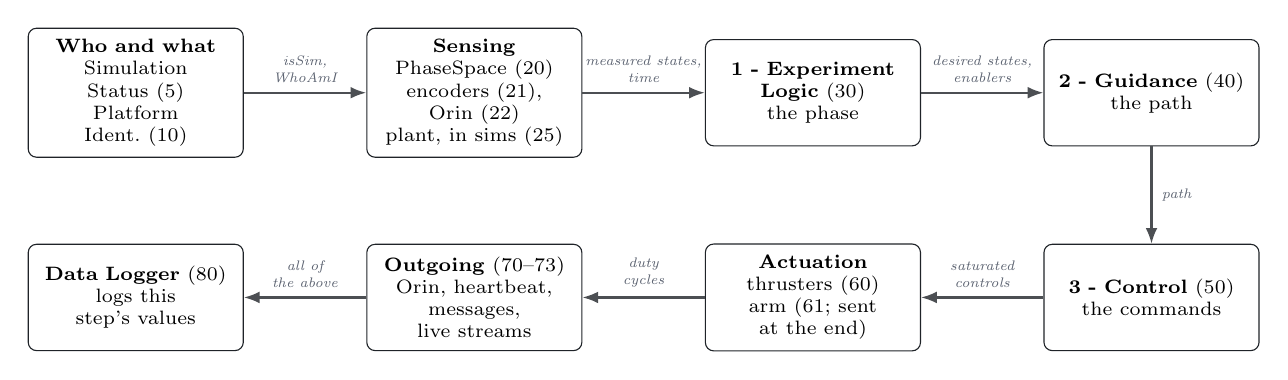
\begin{tikzpicture}[
  st/.style={draw=ink, rounded corners=3pt, align=center, font=\scriptsize, inner sep=4pt, minimum height=1.35cm, text width=2.45cm},
  arr/.style={-{Latex[length=2mm]}, thick, color=ink!80},
  lbl/.style={font=\tiny\itshape, color=muted, align=center}]
  \node[st] (a) at (0, 0)      {\textbf{Who and what}\\ Simulation Status (5)\\ Platform Ident.\ (10)};
  \node[st] (b) at (4.3, 0)    {\textbf{Sensing}\\ PhaseSpace (20)\\ encoders (21), Orin (22)\\ plant, in sims (25)};
  \node[st] (c) at (8.6, 0)    {\textbf{1 - Experiment Logic} (30)\\ the phase};
  \node[st] (d) at (12.9, 0)   {\textbf{2 - Guidance} (40)\\ the path};
  \node[st] (e) at (12.9, -2.6) {\textbf{3 - Control} (50)\\ the commands};
  \node[st] (f) at (8.6, -2.6)  {\textbf{Actuation}\\ thrusters (60)\\ arm (61; sent at the end)};
  \node[st] (g) at (4.3, -2.6)  {\textbf{Outgoing} (70--73)\\ Orin, heartbeat,\\ messages, live streams};
  \node[st] (h) at (0, -2.6)    {\textbf{Data Logger} (80)\\ logs this step's values};
  \draw[arr] (a) -- node[lbl, above]{isSim,\\ WhoAmI} (b);
  \draw[arr] (b) -- node[lbl, above]{measured states,\\ time} (c);
  \draw[arr] (c) -- node[lbl, above]{desired states,\\ enablers} (d);
  \draw[arr] (d) -- node[lbl, right]{path} (e);
  \draw[arr] (e) -- node[lbl, above]{saturated\\ controls} (f);
  \draw[arr] (f) -- node[lbl, above]{duty\\ cycles} (g);
  \draw[arr] (g) -- node[lbl, above]{all of\\ the above} (h);
\end{tikzpicture}
\caption{One step of the diagram, in order (priorities in brackets). Each arrow is a data store written on its
left and read on its right, so every reader runs after its writer.}
\label{fig:steporder}
\end{figure}

\begin{table}[h]
\centering\small
\caption{The top-level subsystems' priorities in the template's diagram.}
\label{tab:priorities}
\begin{tabular}{@{}r >{\raggedright\arraybackslash}p{4.9cm} >{\raggedright\arraybackslash}p{8.6cm}@{}}
\toprule
Priority & Subsystem & Writes (what later subsystems read) \\
\midrule
5  & Simulation Status            & \fn{isSim} \\
10 & Platform Identification      & \fn{WhoAmI} \\
20 & PhaseSpace Camera Code       & \fn{Univ\_Time}, \fn{*\_Measured\_States} (experiments) \\
21 & Manipulator Encoder Data     & \fn{ARM\_Measured\_States}, \fn{ARM\_Measured\_Torque} (experiments; the arm's torques go out at the end of the step) \\
22 & Receive Data from Orin       & \fn{VIS\_Measured\_States}, \fn{VIS\_Confidence} \\
25 & Simulate Plant Dynamics      & \fn{*\_Measured\_States} (simulations); see Section~\ref{sec:plantloop} \\
30 & 1 - Experiment Logic         & \fn{*\_Desired\_States}, enablers, planner selections, \fn{Float\_State} \\
40 & 2 - Guidance                 & the path to follow \\
50 & 3 - Control                  & \fn{*\_Saturated\_Controls}, \fn{ARM\_Controls} \\
60 & Thruster \& Float Control    & duty cycles, Teensy commands \\
61 & Robotic Arm Code             & hands the step's \fn{ARM\_Controls} to the arm's block \\
70--73 & Send Data to Orin, Check Connection, Debugger, Live Data Streams & (outgoing UDP) \\
80 & Data Logger Subsystem        & the ExpLog files (experiments), \fn{dataPacket} (simulations) \\
\bottomrule
\end{tabular}
\end{table}

The same order is used in the program built for the platforms: the generated code runs the subsystems in
this order every step. \emph{Simulate Plant Dynamics} is an \emph{If action} subsystem (it runs only when
its If block says so, i.e.\ in simulations), so it runs where its If block runs: its priority is set on that
If block (and on the Data Store Read of \fn{simMode} that feeds it).

\subsection{Demonstration}
\pth{documentation/demo\_execution\_order.m} builds a tiny diagram in memory (nothing is saved) that works like
SPOT's: ``1~-~Experiment Logic'' writes the phase into a data store and ``3~-~Control'' reads it, with nothing
else connecting them. The phase changes from 0 to 1 at $t = 0.5$\,s; the model runs every 0.1\,s. It simulates
three versions:
\begin{matlab}
addpath('documentation')
demo_execution_order                     % prints the three cases
demo_execution_order('order_demo.pdf')   % and saves the figure below
\end{matlab}
It prints (this is a real run):
\begin{lstlisting}[basicstyle=\ttfamily\scriptsize]
A  virtual subsystems (Simulink picks the order)
   ran first: 1 - Experiment Logic
   warnings:  0
   3 - Control saw phase 1 at t = 0.50 s (in the same step)

B  atomic, priorities wrong way round (Control 30, Logic 50)
   ran first: 3 - Control
   warnings:  1
              - The block '3 - Control/Read phase' is reading from the data store
                'Phase store' before any blocks have written to this entire region
                of memory at time 0.0.
   3 - Control saw phase 1 at t = 0.60 s (1 step late)

C  atomic, priorities in step order (Logic 30, Control 50)
   ran first: 1 - Experiment Logic
   warnings:  0
   3 - Control saw phase 1 at t = 0.50 s (in the same step)
\end{lstlisting}

\begin{figure}[h]
\centering
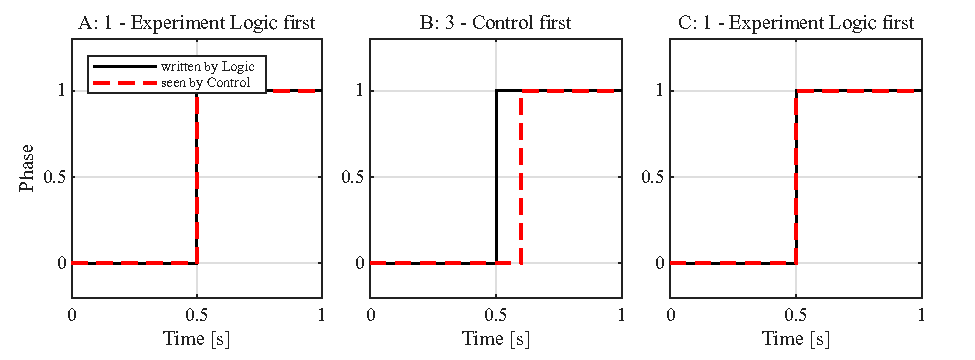
\includegraphics[width=\textwidth]{figures/demo_execution_order.pdf}
\caption{What 3~-~Control saw (dashed) against the phase 1~-~Experiment Logic wrote (solid). In B, Control ran
first, so in every step it read the value from the step before: the change reached it 0.1\,s late.}
\label{fig:orderdemo}
\end{figure}

\begin{description}[leftmargin=1.2em]
  \item[A] is how SPOT's diagram was: virtual subsystems, Simulink's choice. In this tiny model it happened to
        choose the right order. Nothing guarantees that: in SPOT's diagram, with hundreds of blocks, it chose
        Control before Experiment Logic. That is the problem with leaving it to Simulink: it may be right today
        and wrong after an unrelated edit.
  \item[B] forces the wrong order with priorities, to show what it does: Simulink's warning, and Control one
        step behind (Figure~\ref{fig:orderdemo}). This is what SPOT's 2~-~Guidance and 3~-~Control did.
  \item[C] is what SPOT's diagram does now: atomic subsystems, priorities in the order of a step. No warning,
        and Control sees the phase in the step it changes.
\end{description}
In SPOT's own diagram, putting the subsystems in order changed the simulated motion by at most a few
centimetres in the middle of manoeuvres (the phase logic no longer lagging a step), and removed all of
Simulink's data store warnings.

\subsection{The Plant Loop, and Stores That Hold a Value}\label{sec:plantloop}
In a simulation the data stores form a loop: the plant writes the measured states, Control reads them and
writes the commands, and the plant reads the commands (Figure~\ref{fig:plantloop}). In a loop, \emph{one}
store has to be read before it is written in each step, whatever the order. SPOT puts the plant with the
sensing, as PhaseSpace is in an experiment, so Control gets this step's measurements and the plant uses the
previous step's command for one step (as if the command were held). Putting the plant last instead would give
Control the previous step's measurements; the loop has the same one-step delay either way.

\begin{figure}[h]
\centering
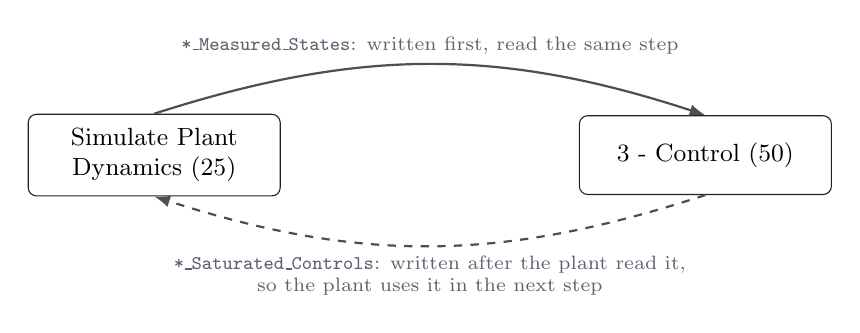
\begin{tikzpicture}[
  st/.style={draw=ink, rounded corners=3pt, align=center, font=\small, inner sep=5pt, minimum height=1cm, minimum width=3.2cm},
  arr/.style={-{Latex[length=2mm]}, thick, color=ink!80},
  lbl/.style={font=\scriptsize, color=muted, align=center}]
  \node[st] (p) at (0, 0) {Simulate Plant\\ Dynamics (25)};
  \node[st] (c) at (7, 0) {3 - Control (50)};
  \draw[arr] (p.north) to[bend left=18] node[lbl, above]{\fn{*\_Measured\_States}: written first, read the same step} (c.north);
  \draw[arr, dashed] (c.south) to[bend left=18] node[lbl, below]{\fn{*\_Saturated\_Controls}: written after the plant read it,\\ so the plant uses it in the next step} (p.south);
\end{tikzpicture}
\caption{The simulated plant's loop. The dashed store is the one read before it is written.}
\label{fig:plantloop}
\end{figure}

Simulink would warn about that store every time, so its check is turned off, on that store only. A few other
stores are also meant to be read while they hold a value. Simulink's check is a setting of each \emph{Data Store
Memory} block (double-click it $\rightarrow$ \ui{Diagnostics}: \ui{Detect read before write}, \ui{Detect write
after read}); for the stores in Table~\ref{tab:stores} it is off, with the reason in the block's
\ui{Description} (right-click $\rightarrow$ \ui{Properties}). For every other store it stays on, so a new
ordering mistake is still reported.

\begin{table}[h]
\centering\small
\caption{The data stores whose ``read before write'' check is off, and why.}
\label{tab:stores}
\begin{tabular}{@{}>{\raggedright\arraybackslash}p{5.3cm} >{\raggedright\arraybackslash}p{9.6cm}@{}}
\toprule
Data stores & Why reading them before (or without) a write is intended \\
\midrule
\fn{*\_Saturated\_Controls}, \fn{ARM\_Controls} & The plant loop above (also ``write after read''). \\
\fn{*\_Desired\_States} & Written only in the phases that use them; they keep their value in between. \\
\fn{WhoAmI}, \fn{VIS\_*}, \fn{ARM\_Measured\_States} & Written only in experiments (or when the arm is simulated); otherwise their initial value. \\
\fn{*\_IMU\_Measurements} & Nothing writes them yet (placeholders the logger records). \\
\bottomrule
\end{tabular}
\end{table}

\subsection{When You Change the Diagram}
\begin{itemize}
  \item \textbf{A new top-level subsystem} that reads or writes data stores: tick \ui{Treat as atomic unit}
        and give it a priority from Table~\ref{tab:priorities} that puts it after what it reads and before what
        reads it (e.g.\ a new sensor 23, an extra guidance step 45). Without one, Simulink places it anywhere.
  \item \textbf{A new data store warning} after a simulation (the console's command window shows ``Simulation
        finished \ldots\ $N$ warnings''; click it): find the reader and the writer it names. If the reader should
        run after the writer, fix the order with priorities. If the reader is meant to see the previous or
        initial value (like Table~\ref{tab:stores}), turn that store's check off and say why in its description.
  \item \textbf{Inside a subsystem}, the same rules apply, one level down: an atomic subsystem orders its own
        blocks by their lines, and you can give its inner atomic subsystems priorities too.
\end{itemize}

% ------------------------------------------------------------------------------------- appendix
\appendix
\section{Function Reference}\label{app:functions}
Every MATLAB function SPOT provides, by package. In MATLAB, \fn{help spot} lists the packages,
\fn{help spot.<package>} a package's functions, and \fn{help spot.<package>.<function>} the details.
Optional inputs are shown in square brackets.

% BEGIN generated function reference
\subsection*{spot.arm \textmd{\textendash\ The Simulated Arm: Servos, Friction, Calibration}}
\begin{xltabular}{\linewidth}{@{}>{\raggedright\arraybackslash\ttfamily\footnotesize}p{0.47\linewidth} >{\raggedright\arraybackslash\small}X@{}}
\toprule \normalfont\small\textbf{Call} & \textbf{Purpose} \\ \midrule \endhead
msgs = spot.arm.checkCommands(dataClass, armModel) & Arm goals the controllers ignore and torques the servos can't give, from a run's log. \\
r = spot.arm.compareSteps(folder, armModel[, show]) & The simulated servos against the real ones, on the calibration's position steps. \\
C = spot.arm.coriolisMatrix(p, x) & Coriolis and centripetal matrix of the Chaser (RED) with its three-link arm. \\
a = spot.arm.defaults() & The simulated arm's servos, their friction and the plant's internal step. \\
M = spot.arm.inertiaMatrix(p, x) & Mass matrix of the Chaser (RED) with its three-link arm, free floating. \\
a = spot.arm.loadCalibration(file, a) & Apply the arm calibration (resources/arm\_calibration/calibrate\_arm.py) to a model. \\
arm = spot.arm.mountGeometry(arm) & The arm's geometry for where it is mounted on the Chaser. \\
a = spot.arm.parameters(v[, root]) & The arm model spot.arm.Plant simulates (the workspace variable armModel). \\
p = spot.arm.Plant('Model', armModel[, 'FixedBase', true]); [pos, vel, torque] = p(F\_RED, jointTorques) & The Chaser with its arm and three Dynamixel servos in current control (with friction), integrated at 1 ms within each diagram step (the RED + ARM Plant block). \\
c = spot.arm.PositionControl('Motor', armModel.motor, 'StepTime', baseRate); tau = c(goal, [q; dq]) & The servos' own position control law (profile, PID), run in the diagram and giving joint torques (the Default Position Control (ARM) block). \\
servo = spot.arm.servoFromDiagram(model, servo) & The simulated servos' limits, from the diagram's arm blocks. \\
c = spot.arm.VelocityControl('Motor', armModel.motor, 'StepTime', baseRate); tau = c(goalSpeeds, [q; dq]) & The servos' own velocity control law (PI), run in the diagram and giving joint torques (the Default Velocity Control (ARM) block). \\
tau = spot.arm.withinLimits(tau, pulses, minPosition, maxPosition) & No joint torque that pushes a joint further beyond its position limits. \\
\bottomrule\end{xltabular}
\subsection*{spot.console \textmd{\textendash\ Starting and Stopping the Local Console}}
\begin{xltabular}{\linewidth}{@{}>{\raggedright\arraybackslash\ttfamily\footnotesize}p{0.47\linewidth} >{\raggedright\arraybackslash\small}X@{}}
\toprule \normalfont\small\textbf{Call} & \textbf{Purpose} \\ \midrule \endhead
spot.console.ensureShell() & Make sure MATLAB's system() has a working shell. \\
exe = spot.console.findPython() & A Python 3.6+ to run the SPOT Console's web server with. \\
{}[ok, message] = spot.console.installPython([dryRun]) & Try to install Python 3 for the SPOT Console (Windows or Linux). \\
exe = spot.console.offerPython() & Ask to install Python when the SPOT Console can't find it; '' if it still can't. \\
url = spot.console.open(root[, show]) & Open (or just show the address of) the project's running SPOT Console. \\
ok = spot.console.openBrowser(url) & Open a URL in the computer's default web browser. \\
removed = spot.console.removeOldLibraryPaths() & Take old Custom\_Library folders off the MATLAB path. \\
url = spot.console.start(root) & Start the SPOT Console for a project and connect this MATLAB session to it. \\
ready = spot.console.status(root) & The project's running SPOT Console (ports and token), or [] if none answers. \\
spot.console.stop(root) & Disconnect the MATLAB worker and stop the project's SPOT Console web server. \\
\bottomrule\end{xltabular}
\subsection*{spot.control \textmd{\textendash\ Controller Design}}
\begin{xltabular}{\linewidth}{@{}>{\raggedright\arraybackslash\ttfamily\footnotesize}p{0.47\linewidth} >{\raggedright\arraybackslash\small}X@{}}
\toprule \normalfont\small\textbf{Call} & \textbf{Purpose} \\ \midrule \endhead
u = spot.control.lqrCommand(K, measured, desired, desiredRate) & The diagram's default LQR control law: forces and torque for one platform, one step. \\
K = spot.control.lqrGains(sys, Q, R) & Discrete LQR gain matrix for a platform. \\
F = spot.control.nominalForces(force) & Thrust of each of the 8 thrusters of a platform. \\
sys = spot.control.stateSpace(mass, inertia, Ts) & Discrete planar rigid-body model of one platform. \\
{}[duty, Fb, H] = spot.control.thrusterDutyCycles(u, theta, thrusterDist, F[, maxIters, tol]) & The diagram's thruster mixer: the 8 thrusters' duty cycles for a force command. \\
report = spot.control.verifyConsoleController(varargin) & Check the lab console's Interactive-mode controller against the diagram. \\
\bottomrule\end{xltabular}
\subsection*{spot.data \textmd{\textendash\ Results: Saved Runs, Signals, 3D Playback, Figures}}
\begin{xltabular}{\linewidth}{@{}>{\raggedright\arraybackslash\ttfamily\footnotesize}p{0.47\linewidth} >{\raggedright\arraybackslash\small}X@{}}
\toprule \normalfont\small\textbf{Call} & \textbf{Purpose} \\ \midrule \endhead
b = spot.data.bodies(ds) & Which platforms (and the arm) a dataset can show on the table. \\
file = spot.data.exportFigure(fig, file[, opts]) & Save a figure for a paper or thesis, as the lab's GetStarted template does. \\
signals = spot.data.flatten(x[, prefix]) & Logged data as one flat struct of timeseries. \\
runs = spot.data.listSaved(root) & What is in the project's ``Saved Data'' folder, for the console's Results page. \\
datasets = spot.data.load(spec, root[, settings]) & Read logged data for the console's Results page and 3D playback. \\
{}[t, y] = spot.data.samples(ts) & Time and data of a logged signal as plain columns. \\
folder = spot.data.saveSimulation(s, root) & Keep the last simulation in ``Saved Data'', next to the experiments. \\
r = spot.data.series(ds, a) & One signal of a dataset, ready to plot in the console. \\
s = spot.data.summary(ds, id) & What the console shows about a loaded dataset (no data). \\
fig = spot.data.toFigure(panels, lookup[, opts]) & The Results page's plots as a MATLAB figure in the lab's publication style. \\
r = spot.data.trajectory(ds[, maxRate]) & A dataset's motion for the console's 3D view. \\
\bottomrule\end{xltabular}
\subsection*{spot.experiment \textmd{\textendash\ Experiments on the Platforms}}
\begin{xltabular}{\linewidth}{@{}>{\raggedright\arraybackslash\ttfamily\footnotesize}p{0.47\linewidth} >{\raggedright\arraybackslash\small}X@{}}
\toprule \normalfont\small\textbf{Call} & \textbf{Purpose} \\ \midrule \endhead
out = spot.experiment.build(s, root) & Build the selected diagram for the platforms, on the lab console (TX2). \\
b = spot.experiment.buildBoard(root[, s]) & Where experiments are built: the lab console (Jetson TX2). \\
info = spot.experiment.connect(root[, password]) & Connect MATLAB to the build board (the TX2), as jetson() does for a platform. \\
files = spot.experiment.decodeData(folder, s, root) & Turn the experiment data files (ExpLog*) into MATLAB timeseries. \\
p = spot.experiment.plan(s, root) & What spot.experiment.build would do, without building anything. \\
\bottomrule\end{xltabular}
\subsection*{spot.hardware \textmd{\textendash\ Code the Spacecraft Program Uses to Talk to Its Hardware}}
\begin{xltabular}{\linewidth}{@{}>{\raggedright\arraybackslash\ttfamily\footnotesize}p{0.47\linewidth} >{\raggedright\arraybackslash\small}X@{}}
\toprule \normalfont\small\textbf{Call} & \textbf{Purpose} \\ \midrule \endhead
\textrm{MATLAB System block} spot.hardware.ArmTorque  (torque) $\rightarrow$ (q, dq, torque, status) & The arm's three Dynamixel servos in current control: reads their encoders and torques before the controllers, sends the joint torques at the end of the step (the Dynamixel Arm (Torque) block). \\
\textrm{MATLAB System block} spot.hardware.CustomDataLogger  (data, size) $\rightarrow$ (none) & Appends each step's logged values to the platform's ExpLog file (the diagram's Data Logger block). \\
\textrm{MATLAB System block} spot.hardware.Debugging  (value) $\rightarrow$ (none) & Prints its input on the platform's console while an experiment runs. \\
spot.hardware.debugMessages(whoAmI, isSim, t, red, black, blue[, labConsoleIP]) & Each platform's debug message, for the SPOT Console's Messages panel. \\
{}[t, state] = spot.hardware.experimentTime(packet, age) & The experiment's time, the same on every platform, from the PhaseSpace stream. \\
\textrm{MATLAB System block} spot.hardware.IdentifyPlatform  () $\rightarrow$ platformId & Which platform the program runs on (1 RED, 2 BLACK, 3 BLUE), from its hostname (the WhoAmI block). \\
s = spot.hardware.ipText(ip) & An IPv4 address as text for the C code: '192.168.1.116' from [192 168 1 116]. \\
spot.hardware.liveStream(label, t, u, whoAmI, isSim[, labConsoleIP]) & Send a signal to the SPOT Console's Live Plot, every step (the Live Stream block). \\
packet = spot.hardware.packCommand(duty, pucks) & The 37-byte command packet for a platform's Teensy (8 thruster duty cycles and the pucks). \\
{}[packet, newPackets, age] = spot.hardware.phasespaceLatest(port, senderIP) & The newest PhaseSpace packet every model step, for the diagram's ``Receive PhaseSpace Data'' block. \\
label = spot.hardware.streamName(block, name) & The name a Live Stream block shows in the SPOT Console's Live Plot. \\
name = spot.hardware.Udp(\textasciitilde{}) & Connects csrc/udp/spot\_udp.c to the generated code (used by the UDP functions here). \\
{}[data, newPackets, age] = spot.hardware.udpReceive(port, senderIP, n, type) & Newest UDP packet every model step (replaces the UDP Receive block). \\
spot.hardware.udpSend(ip, port, data) & Send a signal as one UDP packet every model step (replaces the UDP Send block). \\
\bottomrule\end{xltabular}
\subsection*{spot.massprops \textmd{\textendash\ Mass Properties}}
\begin{xltabular}{\linewidth}{@{}>{\raggedright\arraybackslash\ttfamily\footnotesize}p{0.47\linewidth} >{\raggedright\arraybackslash\small}X@{}}
\toprule \normalfont\small\textbf{Call} & \textbf{Purpose} \\ \midrule \endhead
I = spot.massprops.bifilarInertia(mass, T, L, D) & Moment of inertia from a bifilar (two-string) pendulum test. \\
r = spot.massprops.centerOfGravity(scales) & Mass, centre of gravity, thruster offsets and LED positions from scale readings. \\
r = spot.massprops.compute(mass) & Mass properties of RED, BLACK and BLUE from the settings' mass section. \\
text = spot.massprops.trackerPositions(props) & PhaseSpace marker calibration text from the computed mass properties. \\
file = spot.massprops.writeTrackerPositions(props, root) & Write resources/tracker\_positions\_phasespace.txt for the PhaseSpace server. \\
\bottomrule\end{xltabular}
\subsection*{spot.params \textmd{\textendash\ Settings}}
\begin{xltabular}{\linewidth}{@{}>{\raggedright\arraybackslash\ttfamily\footnotesize}p{0.47\linewidth} >{\raggedright\arraybackslash\small}X@{}}
\toprule \normalfont\small\textbf{Call} & \textbf{Purpose} \\ \midrule \endhead
d = spot.params.apply(s[, root]) & Put the settings into the base workspace, as the Simulink diagrams expect them. \\
s = spot.params.defaults() & Default SPOT settings. \\
s = spot.params.fromLegacyState(file) & Convert a GUI state file saved by the old SPOT GUI (Save GUI State) to settings. \\
ip = spot.params.ipv4(address) & An IPv4 address as four numbers: [192 168 1 116] from '192.168.1.116'. \\
s = spot.params.load(file) & Read settings from a JSON file, filling anything missing with the defaults. \\
c = spot.params.loadCalibration(root) & The project's calibration of the lab (resources/spot\_calibration.json). \\
s = spot.params.merge(base, changes) & Copy the fields of CHANGES over BASE, recursing into structs. \\
n = spot.params.platformSelection(p) & The diagrams' platformSelection code for a set of platforms. \\
{}[s, backup] = spot.params.reset(current, root, settingsFile, backupFolder) & The template's default settings, keeping the diagram, after backing up the settings file. \\
spot.params.save(s, file) & Write settings to a JSON file (readable, and diff-friendly in version control). \\
t = spot.params.timing(s) & Phase durations, end times and total time from the settings. \\
s = spot.params.update(old, changes, root) & New settings from the console: the defaults overlaid with what the page sent, re-reading the solver for a new diagram. \\
\bottomrule\end{xltabular}
\subsection*{spot.plotting \textmd{\textendash\ Drawing}}
\begin{xltabular}{\linewidth}{@{}>{\raggedright\arraybackslash\ttfamily\footnotesize}p{0.47\linewidth} >{\raggedright\arraybackslash\small}X@{}}
\toprule \normalfont\small\textbf{Call} & \textbf{Purpose} \\ \midrule \endhead
P = spot.plotting.armPosition(base, q, arm) & Joint positions of the robotic arm on RED, in the table frame. \\
links = spot.plotting.drawArm(joints) & Outlines of the arm's three links, for publication figures. \\
pts = spot.plotting.drawSpacecraft(x, y, theta, id) & Outline of a SPOT platform on the table, for publication figures. \\
{}[name, color] = spot.plotting.platformStyle(key) & What a platform is called and its colour in figures. \\
L = spot.plotting.signalLabel(name) & Readable name and unit of a logged signal, for figure labels. \\
\bottomrule\end{xltabular}
\subsection*{spot.sim \textmd{\textendash\ Simulations}}
\begin{xltabular}{\linewidth}{@{}>{\raggedright\arraybackslash\ttfamily\footnotesize}p{0.47\linewidth} >{\raggedright\arraybackslash\small}X@{}}
\toprule \normalfont\small\textbf{Call} & \textbf{Purpose} \\ \midrule \endhead
out = spot.sim.debugLog(platform, t, codes) & The platforms' debug messages recorded during a simulation (by spot.hardware.debugMessages). \\
d = spot.sim.errorDetails(err[, root]) & An error's root cause, the blocks involved and the full report, as plain text. \\
names = spot.sim.listDiagrams(root) & Simulink diagrams (.slx) in the project folder. \\
out = spot.sim.liveData(name, t, v) & The Live Stream blocks' signals recorded during a simulation (by spot.hardware.liveStream). \\
model = spot.sim.loadDiagram(diagram, root) & Load a diagram from the project folder (without opening its window). \\
name = spot.sim.modelName(diagram) & Simulink model name of a diagram file ('Template.slx' -> 'Template'). \\
solver = spot.sim.readSolver(diagram, root, solver) & Copy a diagram's own solver settings into the settings' solver section. \\
r = spot.sim.results(dataClass, s[, d, maxRate]) & Trajectory of a simulation for the SPOT Console's 3D view. \\
out = spot.sim.run(s, root[, resultFile]) & Simulate the selected diagram with the given settings. \\
block = spot.sim.showBlock(diagram, root, block) & Open a diagram at a block and highlight it (e.g. the block an error is in). \\
obj = spot.sim.SimulationFailed(original, output) & The error spot.sim.run throws when Simulink stops a simulation with an error. \\
a = spot.sim.tableSlope(position, velocity, slope, damping) & The table's pull on a floating platform: its slope and the air bearings' drag. \\
\bottomrule\end{xltabular}
\subsection*{spot.worker \textmd{\textendash\ The MATLAB Worker That Runs the Console's Commands}}
\begin{xltabular}{\linewidth}{@{}>{\raggedright\arraybackslash\ttfamily\footnotesize}p{0.47\linewidth} >{\raggedright\arraybackslash\small}X@{}}
\toprule \normalfont\small\textbf{Call} & \textbf{Purpose} \\ \midrule \endhead
w = spot.worker.start(port, token, root) & Connect a MATLAB worker to the SPOT Console's web server. \\
spot.worker.stop() & Disconnect the MATLAB worker from the SPOT Console (if one is running). \\
w = spot.worker.Worker(root); result = w.dispatch(cmd, args); w = spot.worker.Worker.instance() & Runs the console's MATLAB commands in this session (the commands are listed in Appendix~B). \\
\bottomrule\end{xltabular}
\subsection*{spot.workspace \textmd{\textendash\ The Console's Workspace Panel and Command Window}}
\begin{xltabular}{\linewidth}{@{}>{\raggedright\arraybackslash\ttfamily\footnotesize}p{0.47\linewidth} >{\raggedright\arraybackslash\small}X@{}}
\toprule \normalfont\small\textbf{Call} & \textbf{Purpose} \\ \midrule \endhead
r = spot.workspace.evaluate(command) & Run a command in the base workspace and capture what it prints. \\
r = spot.workspace.inspect(expr) & Details of a workspace variable (or a field of one) for the Workspace panel. \\
vars = spot.workspace.list() & The base workspace's variables, as MATLAB's Workspace browser shows them. \\
t = spot.workspace.preview(x) & Short text for a value, like the Value column of MATLAB's Workspace browser. \\
\bottomrule\end{xltabular}
\section{The Console's Commands and the Non-MATLAB Parts}
The local console asks MATLAB for everything through \fn{spot.worker.Worker.dispatch(cmd, args)}; each command calls the functions above.
\begin{xltabular}{\linewidth}{@{}>{\raggedright\arraybackslash\ttfamily\footnotesize}p{0.36\linewidth} >{\raggedright\arraybackslash\small}X@{}}
\caption*{Commands of the local console (\fn{dispatch}).}\\
\toprule \normalfont\small\textbf{Command} & \textbf{Purpose} \\ \midrule \endhead
ping, info & Check that MATLAB answers; its release and toolboxes. \\
settings.get, settings.set & Read or replace the settings (spot.params.update), then apply them. \\
settings.reset & Back to the defaults (spot.params.reset). \\
settings.open, settings.saveAs & Load or save settings through MATLAB's file dialogs. \\
diagram.open & Open the diagram in Simulink. \\
sim.run, sim.stop & Run the simulation (spot.sim.run), or stop it. \\
experiment.plan, .connect, .build & spot.experiment.plan, connect and build. \\
experiment.decode & Convert collected ExpLog files (spot.experiment.decodeData). \\
data.list, data.load, data.unload & Saved Data, and the datasets loaded for the Results tab (spot.data.listSaved, load). \\
data.series, data.trajectory & A signal to plot, or a dataset's motion for the 3D view (spot.data.series, trajectory). \\
data.saveSimulation, data.figure & Save the last simulation; draw or export the plots (spot.data.toFigure, exportFigure). \\
massprops.writeTracker & Write the PhaseSpace marker calibration (spot.massprops.writeTrackerPositions). \\
workspace.list, .inspect, .eval & The Workspace panel and the command window (spot.workspace.*). \\
\bottomrule\end{xltabular}
\begin{xltabular}{\linewidth}{@{}>{\raggedright\arraybackslash\ttfamily\footnotesize}p{0.40\linewidth} >{\raggedright\arraybackslash\small}X@{}}
\caption*{The non-MATLAB parts.}\\
\toprule \normalfont\small\textbf{File} & \textbf{Purpose} \\ \midrule \endhead
+spot/\allowbreak{}+console/\allowbreak{}webapp/\allowbreak{}app.py & Starts the console's web server: \texttt{--local} for the local console (SPOT does this), otherwise the hardware console (the TX2's service). \\
webapp/\allowbreak{}spot\_console/\allowbreak{}common.py & Paths, the API error, checking values from requests. \\
webapp/\allowbreak{}spot\_console/\allowbreak{}events.py & The console's own settings, the event stream to every open page, running commands. \\
webapp/\allowbreak{}spot\_console/\allowbreak{}phasespace.py & Compiling and running StreamData, decoding its packets for the 3D view, marker calibration. \\
webapp/\allowbreak{}spot\_console/\allowbreak{}hardware.py & Teensy packets and the SSH links to the platforms: pucks, thrusters, thruster checks. \\
webapp/\allowbreak{}spot\_console/\allowbreak{}control.py & The diagram's default LQR law and thruster mixer in Python (spot.control.lqrCommand and thrusterDutyCycles, ported line by line), for Interactive Mode. \\
webapp/\allowbreak{}spot\_console/\allowbreak{}interactive.py & Interactive Mode: flies one or more platforms to their goals from the PhaseSpace stream, each with its own loop, controller process and safety stops. \\
webapp/\allowbreak{}spot\_console/\allowbreak{}experiment.py & Deploying, starting, stopping and collecting experiments on the platforms. \\
webapp/\allowbreak{}spot\_console/\allowbreak{}local.py & The local console: the MATLAB link, simulation and build runs, the link to the lab console. \\
webapp/\allowbreak{}spot\_console/\allowbreak{}files.py & The folder browser. \\
webapp/\allowbreak{}spot\_console/\allowbreak{}design.py & The Spacecraft Designer's design (docking cone and solar panels on each platform): checked and kept in a JSON file. \\
webapp/\allowbreak{}spot\_console/\allowbreak{}calibration.py & The Calibration tab: the calibration file (the lab's, and each project's copy), and the calibrations, which drive a platform (the table's slope from drifts). \\
webapp/\allowbreak{}spot\_console/\allowbreak{}calfit.py & The calibrations' fits (linear least squares on the measured positions): the table's height surface and drag, each thruster's thrust. \\
webapp/\allowbreak{}spot\_console/\allowbreak{}server.py & The web API and start-up. \\
webapp/\allowbreak{}static/\allowbreak{} & The page: app.js (common), sim.js, experiment.js, results.js, hardware.js, interactive.js (Interactive Mode), designer.js (Spacecraft Designer), calibration.js and calviz.js (Calibration), viewer.js (3D), cad.js (Use CAD), data.js. \\
+spot/\allowbreak{}+console/\allowbreak{}phasespace/\allowbreak{}StreamData.cc & Reads PhaseSpace and streams positions to the platforms (UDP 31534); built with its Makefile or build\_linux.sh. \\
+spot/\allowbreak{}+console/\allowbreak{}deploy/\allowbreak{}deploy\_tx2.sh & Installs the console on the TX2 and (re)starts its service (spot-phasespace-console.service). \\
+spot/\allowbreak{}+console/\allowbreak{}deploy/\allowbreak{}setup\_hardware\_link.sh & Installs the platform agent on RED/BLACK/BLUE and gives the TX2 access to it. \\
+spot/\allowbreak{}+console/\allowbreak{}deploy/\allowbreak{}spot\_agent.sh & The only thing the TX2 may run on a platform: status, stream, exp-receive, exp-start, exp-stop, exp-status, exp-data, exp-clean. \\
+spot/\allowbreak{}+hardware/\allowbreak{}csrc/\allowbreak{} & C/C++ behind the hardware blocks (arm/arm\_torque.cpp for the arm, WhoAmI, Data Logger, Debugging, PhaseSpace receiver). \\
+spot/\allowbreak{}+hardware/\allowbreak{}arm/\allowbreak{} & setup\_arm\_serial.sh: on RED, the U2D2 adapter's 1 ms latency timer and permissions (a udev rule). \\
+spot/\allowbreak{}+hardware/\allowbreak{}teensy/\allowbreak{} & The Teensy firmware (teensy\_pwm\_control.ino) and setup\_teensy\_serial.sh. \\
\bottomrule\end{xltabular}
% END generated function reference

\end{document}
